%===============================================================================
% Bayesian Variable-order Markov Models
% Kevin Durant
% January 2020
%
% The purpose of this article is to demonstrate an interest I have in model
% selection problems, and to show my familiarity with Bayesian techniques and
% their implementations. Although the problem being addressed here has to do
% with variable-order Markov models, I am by no means an expert in this field; I
% simply became familiar with the information-theoretic foundations of these
% models and recognised that they could also be treated in an elementary
% Bayesian way.
%
% The work discussed here might not be directly applicable to any real-world
% problems, but I believe it gives a good representation of the types of
% computer science, statistics, and mathematics problems that interest me. I
% think it is also fair to say that the technical level of what is shown here is
% roughly representative of that which I have been doing as part of my day job
% for the last few years. (To be clear though, this work was done on my own
% time, outside of working hours.)
%===============================================================================

\documentclass[11pt,a4paper]{article}

\usepackage[width=140.1mm,height=227.2mm,left=35mm,top=26.3mm]{geometry}
\usepackage{microtype}
\usepackage{mathtools} % also loads amsmath.
\usepackage{iftex}
\ifPDFTeX
  \usepackage[T1]{fontenc}
  \usepackage[utf8]{inputenc}
  \usepackage{amssymb}
\else
  % Load after other font- or maths-related packages (loads amsmath and fontspec
  % if necessary). Sets a custom version of Latin Modern Math by default.
  \usepackage{unicode-math}
  % \setmainfont{XITS}
  % \setmathfont{XITS Math}
  % \setmainfont{STIX Two Text}
  % \setmathfont{STIX Two Math}
\fi
\usepackage{booktabs} % better-looking tables.
\usepackage{pgfplots}
\usepackage{biblatex}
\usepackage{hyperref}

% Package settings %============================================================

\usepgfplotslibrary{fillbetween,statistics}
\pgfplotsset{compat=1.16,width=0.75\textwidth}
\pgfplotsset{every axis plot/.append style={very thick}}
\definecolor{cbblue}{RGB}{31,119,180}
\definecolor{cborange}{RGB}{255,127,14}
\addbibresource{bvmm.bib}

% Custom maths commands %=======================================================

\newcommand\ds{\displaystyle}                 % large maths.
\newcommand\ts{\textstyle}                    % small maths.
\newcommand\mb[1]{\mathbb{#1}}                % mathbb shorthand.
\newcommand\mc[1]{\mathcal{#1}}               % mathcal shorthand.
\newcommand\ub[1]{\symbf{#1}}                 % unicode-math symbf shorthand.
\newcommand\ff[1]{^{\underline{#1}}}          % falling factorial.
\newcommand\rf[1]{^{\overline{#1}}}           % rising factorial.
\newcommand\ul[1]{\underline{#1}}             % underline.
\newcommand\ol[1]{\overline{#1}}              % overline.
\DeclareMathOperator\Pb{P}                    % probability.
\DeclareMathOperator\Ex{E}                    % expected value.
\DeclareMathOperator\Va{V}                    % variance.
\DeclarePairedDelimiter\lr{\lparen}{\rparen}  % sized parentheses.
\DeclarePairedDelimiter\lrb{\lbrack}{\rbrack} % sized brackets.
\DeclarePairedDelimiter\abs{\lvert}{\rvert}   % absolute value symbol.
\DeclarePairedDelimiter\cl{\lceil}{\rceil}    % ceiling symbol.
\DeclarePairedDelimiter\fl{\lfloor}{\rfloor}  % floor symbol.

% Document-specific maths commands %============================================

\newcommand\ind{\perp\!\!\!\perp}        % conditional independence.
\newcommand\peq{\mathop{=}}              % tight equals (used in probabilities).
\DeclareMathOperator\cat{Cat}            % categorical distribution.
\DeclareMathOperator\dir{Dir}            % Dirichlet distribution.
\DeclareMathOperator*{\argmax}{arg\,max}

% Title %=======================================================================

\title{An Application of Markov Chain Monte Carlo Methods to Variable-order
  Markov Models}
\author{Kevin Durant}
\date{}

% Document %====================================================================

\begin{document}

\maketitle

\begin{abstract}
This article describes the solution of a certain `toy' problem: the
implementation of a Markov chain Monte Carlo sampler over the space of
variable-order Markov models. The goal of the sampling process is to identify
Markovian dependencies in a sequence of data, with the aim of using these
dependencies to explain the underlying data-generating process. The approach
outlined here adheres closely to the principles of Bayesian inference, and makes
use of both analytical and numerical techniques. A few interesting tangential
problems are briefly discussed as well.
\end{abstract}

\section{Introduction} %========================================================

During recent work on a problem that involved temporal networks (in which the
underlying edge events are all timestamped, and thus ordered), a peripheral
question arose that seemed worth trying to answer: `Are there nodes in
the network whose outgoing edges can be predicted based on their most recent
incoming edge? And if so, to what depth?'

Dependencies such as these are interesting in the context of communication
networks because they point to the presence of certain message-passing `chains'.
For example, it might be the case that whenever a node~\(v\)'s most recent
incoming message originated at node~\(u\), the next message sent by~\(v\) is
likely to be to some third node~\(w\). If this is not the usual behaviour for
messages sent from~\(v\), then the distribution of its outgoing edges is
conditionally dependent on its last incoming edge. We would be interested in
determining, for a given network, to what extent (if any) these dependencies
hold.

The same problem can also be reframed and asked of any form of sequential data,
as long as the symbols that make up the sequence come from a discrete set (text
documents, for example, are permissible, but real-valued time series are not).
Given a sequence of symbols~\(x_1, x_2, \dots\), the objective is to find
subsequences~\(x_{n-k}, \dots, x_n\) that allow the following symbol~\(x_{n+1}\)
to be predicted with a better-than-random success rate. We can then
regard~\(x_n\) as conditionally dependent on its~\(k\) predecessors (when those
predecessors match the subsequence~\(x_{n-k}, \dots, x_{n-1}\)) for the purpose
of predicting the symbol that follows.

The obvious probabilistic framework to adopt when approaching this problem is
that of Markov chains, since there is a deterministic progression between
states, and each state is associated with a unique probability distribution. Our
interest, however, is not in the parameters of these probability distributions
or how they may be used to predict new symbols, but rather in the likelihood of
a particular model, or set of Markov states.

Probabilistically, we are concerned with the posterior distribution over all
possible models, rather than over the parameters of a specific model (although
the latter is required to derive the former properly). Since each Markov model
is simply a set of subsequences (states) that are used to describe the
data-generating process, by performing inference on the set of models we are
implicitly searching for subsequences that may be particularly significant to
this underlying process.

\subsection{Motivation} %=======================================================

I have referred to the problem being treated here as a `toy', or introductory,
problem because it is being addressed primarily for the sake of interest. In
particular, the goal here is not to develop a state-of-the-art prediction
algorithm, but rather to carry out a reasonably complete course of Bayesian
inference in the hopes of being able to uncover and interpret Markovian
dependencies in a given set of data.

There are two characteristics of this problem that make it particularly
attractive from an introductory point of view. Firstly, the marginal likelihood
of a given variable-order Markov model can be expressed in closed form (by
leveraging the fact that the categorical distribution has a conjugate prior in
the Dirichlet distribution), allowing one to focus directly on the model
posterior. Secondly, every variable-order Markov model can be viewed as a simple
tree, and a Markov chain Monte Carlo simulation that samples over the space of
possible models may do so simply by proposing moves that either attach new nodes
to or remove existing nodes from the current tree.

These two characteristics---along with the fact that all of the distributions
dealt with here are discrete---allow us to treat the problem in a fully Bayesian
way without incurring the level of technicality that is usually associated with
this sort of inference; touching on both the theoretical and practical aspects
of the Bayesian approach in the process. The principled manner in which the
problem is solved can also be applied directly to more complex
problems---although in the case of intractable posterior distributions one will
need to turn to more advanced techniques (e.g., reversible-jump Markov chain
Monte Carlo~\cite{green1995reversible}). 

As with most mathematical problems, the process of working out a solution gives
rise to several new problems that are of interest in their own right. The
situation is no different here, and in Sections~\ref{sec:independence}
and~\ref{sec:asymptotic} some attention is given to a pair of topics that follow
quite logically from the marginal likelihood derivation and Markov chain Monte
Carlo evaluation portions of this work. These two topics are: the relationship
between Markov states and probabilistic independence, and the asymptotic rate of
decay of Bayes factors in the case of uniformly random data.

The following section describes the model inference problem in more detail,
along with the methods used to solve it. For experimental results involving a
number of synthetic and real-world data sets, the reader may consult
Section~\ref{sec:experiments}.

\section{Methodology} %=========================================================

Let \(\ub{x} = x_1, x_2, \dotsc\) be a sequence of random variables. For the
purpose of inference we assume that the process that generates \(\ub{x}\) is
Markovian, and that the state that any symbol~\(x_n\) depends on is some
function of the preceding values~\(x_1, \dots, x_{n-1} = \ub{x}_{1:n-1}\). Every
state is associated with a discrete probability distribution over the symbol
alphabet~\(\mc{A}\), and it is according to these distributions that the
sequence is generated.

A set of states~\(\mc{S}\) defines a Markov model that can be used to fit the
data, and to some extent the states of such a model are a description of the
dependence (or independence) relationships among the random variables. Consider
the trivial case \(\mc{S} = \{\lambda\}\), in which every symbol is generated
based on the same state~\(\lambda\) regardless of their predecessors. In this
case there is a single, common distribution, and every symbol~\(x_n\) is
obviously independent of its predecessors:
\begin{equation*}
  \Pb\lr{x_n, \ub{x}_{1:n-1} \mid \mc{S}} =
    \Pb\lr{x_n \mid \mc{S}} \Pb\lr{\ub{x}_{1:n-1} \mid \mc{S}}.
\end{equation*}
Note however that \(x_n\) is only \emph{conditionally} independent of the other
symbols in light of the particular model~\(\mc{S}\), and that different models
may suggest different dependencies. For example, let \(\mc{S} = \{\lambda,
a\}\), and assume that the state of a subsequence~\(\ub{x}_{1:n-1}\) is \(a\) if
\(x_{n-1} = a\) and \(\lambda\) otherwise. In this case \(x_n\) is not
necessarily independent of \(x_{n-1}\), because
\begin{equation*}
  \Pb\lr{x_n, x_{n-1} \peq a \mid \mc{S}} =
    \Pb\lr{x_n \mid x_{n-1} \peq a, \mc{S}} \Pb\lr{x_{n-1} \peq a \mid \mc{S}},
\end{equation*}
and \({\Pb(x_n \mid x_{n-1} \peq a, \mc{S})}\) will in general not be equal to
\(\Pb(x_n \mid \mc{S})\) for all possible values of \(x_n\).

The idea here is to define a set of models~\(\mc{M}\) that covers as many of the
dependence/independence relationships among the sequence's random variables as
possible. Assuming one has access to the marginal likelihood (also referred to
as the \emph{evidence}) corresponding to each model, one can then perform model
comparison to get an idea of which variables are likely independent of one
another given the space of potential models.

Ideally, one would like to ask and answer the exact question `What is the
probability that~\(x_n\) is independent of~\(x_{n-1}\) given~\(\mc{M}\)?',
however doing so is beyond the scope of this text (although we do return to it
briefly in Section~\ref{sec:independence}). A second, related question is `What
is the probability that state \({x_{n-1} = a}\) is present in the ``true''
underlying Markov model~\(\mc{S}^*\)?' This latter question---which is closely
tied to model selection---is the focus here.

The probabilities being asked for above are marginal probabilities of individual
states, and follow directly from the posterior distribution over the space of
models. Although we may be able to derive the marginal likelihood of any single
model~\(\mc{S}\), this only allows us to compare the likelihoods of individual
models---not necessarily to compute their normalised probabilities with respect
to \emph{all} other possible models. By making use of Markov chain Monte
Carlo~(MCMC) methods, we can sample from the desired posterior distribution
using only relative marginal likelihoods, and then use the resulting sample set
as an approximate representation of the true posterior.

As mentioned above, every model in the set~\(\mc{M}\) is a set of Markov states,
which are derived from subsequences in the data set. The states we restrict
ourselves to here are those that result from permuting the
subsequence~\(\ub{x}_{1:n-1}\) and then truncating all but its last \(k\)
symbols: \(f(\ub{x}_{1:n-1}) = x_{\phi(n-k)}, \dots, x_{\phi(n-1)}\). In the
simplest case---the identity permutation---states are nothing but simple
prefixes of length~\(k\), where~\(k\) depends on the symbols in the subsequence.

Any set of prefixes of this form can be arranged in a tree in which they appear
as the leaves: let the root node represent the empty prefix (a valid state), its
children the single-symbol states~\({\{\,x_{n-1} = a : a \in \mc{A}\,\}}\), and
so on. The mapping~\(f(\ub{x}_{1:n-1})\) can then be thought of as a search for
the leaf node whose root-leaf path matches the given sequence. A complete tree
of depth~\(k\) corresponds to a \(k\)th-order Markov model; by considering
incomplete trees as well, we obtain \emph{variable}-order Markov models, in
which the state function~\(f\) is able to yield prefixes of arbitrary length
according to the root-leaf paths in the tree.

To avoid the situation in which a subsequence~\(\ub{x}_{1:n-1}\) cannot be
mapped to a leaf node of the state tree (this can occur when considering the
first few variables in the sequence, whose prefixes are very short), we consider
every node in the tree to be a valid state. An alternative strategy would be to
invent symbols so as to extend the prefix to a leaf node (this was the approach
used by Rissanen~\cite{rissanen1986complexity} in the early development of
variable-order Markov models).

Our final set of models~\(\mc{M}\) is thus the set of all possible \(M\)-ary
trees, where~\(M\) is the cardinality of the symbol alphabet~\(\mc{A}\). The
trees in~\(\mc{M}\) need neither be full nor complete. As mentioned above, every
such model~\(\mc{S} \in \mc{M}\) suggests a dependence structure for the random
variables in the sequence, the details of which are given by the unknown
conditional distributions~\(\Pb(x_n \mid \ub{x}_{1:n-1} = s)\) for each
state~\(s \in \mc{S}\).

For the purposes of prediction, compression, or parameter estimation, one would
usually select a single model~\(\mc{S}\) believed to be sufficient for
capturing all of the dependencies that may be present in the data. One would
then attempt to infer the conditional distributions~\(\Pb(x_n \mid s)\) in some
way, taking measures to avoid overfitting if necessary. Assuming that this
problem can be solved to some reasonable degree---perhaps yielding a maximum
likelihood solution, or a posterior distribution over the space of possible sets
of distributions, or a representative sample from this posterior---one can then
proceed a step further, and begin to compare the appropriateness of different
models from the set~\(\mc{M}\). The reason for doing so might be to perform
model selection or model averaging to improve the accuracy of prediction, or
(and this is our goal here) one may simply want to compare models for the sake
of better understanding the underlying process that generated the data. In our
specific case, we hope to have constructed our set of models in such a way that
their relative likelihoods will allow us to infer which sequences of symbols
have a significant effect on their immediate successors.

The form of Markov model we have described here is intended to be minimal, in
the sense that it encodes the effect of a symbol's prefix and nothing more. If a
symbol~\(x_n\) is generated by some other mechanism that is in fact independent
of the prefix~\(x_{n-k}, \dots, x_{n-1}\), then models that include this state
should lead to lower marginal likelihoods than those that do not. Conversely, if
we find that this node appears regularly among the state trees (relative to the
posterior distribution over \(\mc{M}\)), we may conclude that the occurrence of
the prefix~\(\ub{x}_{n-k:n-1}\) in the data can to some extent be used to
predict the symbols that will follow. This Markovian dependence may take
different forms: it might be that \(x_n\) depends solely on a symbol \(m\) steps
prior,~\(x_{n-m}\), or it may be that the entire prefix has an influence. These
dependencies can all be described within the state tree framework, but some may
require a clever choice of the permutation function~\(\phi\).

There are now two problems that must be solved: first we must infer the
conditional distributions~\(\{\,\Pb(x_n \mid s) : s \in \mc{S}\,\}\), and then
we must use this information to compare the relative (marginal) likelihoods of
the models in~\(\mc{M}\). Before doing so, however, we elaborate slightly on the
previous paragraph by pointing out that it is somewhat difficult to infer true
conditional independence from Markov state trees.

\subsection{Independence probabilities}\label{sec:independence} %===============

Consider the two simple models that were used as examples at the start of the
previous section: \(\mc{S}_{\lambda} = \{\lambda\}\) and~\(\mc{S}_a = \{\lambda,
a\}\). As mentioned there, \(\mc{S}_{\lambda}\) explicitly models every random
variable~\(x_n\) as conditionally independent of its predecessor~\(x_{n-1}\),
whereas~\(\mc{S}_a\) does not:
\begin{align*}
  \Pb(x_n, x_{n-1} \peq a \mid \mc{S}_{\lambda}) &=
    \Pb(x_n \mid \lambda) \Pb(x_{n-1} \peq a \mid \lambda), \\
  \Pb(x_n, x_{n-1} \peq a \mid \mc{S}_a) &=
    \Pb(x_n \mid a) \Pb(x_{n-1} \peq a \mid \mc{S}_a).
\end{align*}
The point we make here is that although the second model may not explicitly
model \(x_n\) and~\(x_{n-1}\) as conditionally independent, it also does not
\emph{always} model them as dependent.

The reason for this is that every concrete Markov model is more than simply a
set of states---associated with each state is a probability distribution over
the possible values of the next random variable. In the case of the second
model~\(\mc{S}_a\), there are two such distributions: \(\Pb(x \mid \lambda)\)
and~\(\Pb(x \mid a)\), which will in general not be equal. If, however, they
are---i.e., if they both equal the marginal distribution~\(\Pb(x) \mid
\mc{S}_a\)---then the model reduces to~\(\mc{S}_{\lambda}\), in which all random
variables are modelled as conditionally independent of one another.

This raises a question about the model-selection approach outlined in the
previous section, where we stated that our plan is to draw samples from the
posterior distribution over Markov models (or more accurately, Markov model
\emph{trees}---because we will have marginalised out their parameters) and then
use these sampled models to get an idea of the dependencies that are present in
the data-generating process; this question is `To what extent can the
dependencies that appear in the model posterior be used to infer actual
\emph{probabilities} of conditional dependence?'

We will not answer this question here; we will, however, show that the model
posterior can in theory be used to do so. Consider the two
models~\(\mc{S}_{\lambda}\) and~\(\mc{S}_a\) again: if these are the only two
possible models, and we assume that one of them is `true', then the probability
that~\(x_n\) is conditionally independent of~\(x_{n-1} = a\) can be expressed as
the probability that~\(\mc{S}_{\lambda}\) is true (in which case the variables
are independent regardless of the model's parameters), plus the probability
that~\(\mc{S}_a\) is true \emph{and} the model's two distributions are
identical. Written out, this is:
\begin{align*}
  \Pb(x_n \ind x_{n-1} \peq a \mid \ub{x}, \mc{M}) &=
    \Pb(\mc{S}_{\lambda} \mid \ub{x}) + \Pb(\mc{S}_a \mid \ub{x})
    \Pb(x_n \perp x_{n-1} \peq a \mid \ub{x}, \mc{S}_a) \\
  &= \Pb(\mc{S}_{\lambda} \mid \ub{x}) + \Pb(\mc{S}_a \mid \ub{x})
    \Pb\lr*{\theta_{\lambda} = \theta_a \mid \ub{x}, \mc{S}_a},
\end{align*}
where~\(\theta_{\lambda}\) and~\(\theta_a\) are the parameters of the
state-dependent distributions that define \(\mc{S}_a\). The posterior model
probabilities~\(\Pb(\mc{S} \mid \ub{x})\) are the result of the MCMC sampling
process. The remaining parameter term can be derived via Bayes' rule:
\begin{align*}
  \Pb(\theta_{\lambda} = \theta_a \mid \ub{x}, \mc{S}_a) &=
    \frac{\Pb(\ub{x} \mid \theta_{\lambda} = \theta_a, \mc{S}_a)
    \Pb(\theta_{\lambda} = \theta_a \mid \mc{S}_a)}
    {\Pb(\ub{x} \mid \mc{S}_a)} \\
  &= \frac{\int_{\theta_{\lambda}=\theta_a}
    \Pb(\ub{x} \mid \theta_{\lambda}, \theta_a, \mc{S}_a) \Pb(\theta_{\lambda})
    \Pb(\theta_a)\, d\theta_{\lambda} d\theta_a}{\Pb(\ub{x} \mid \mc{S}_a)} \\
  &= \frac{\int_{\theta_{\lambda}}
    \Pb(\ub{x} \mid \theta_{\lambda}, \mc{S}_{\lambda})
    \Pb(\theta_{\lambda})^2\, d\theta_{\lambda}}{\Pb(\ub{x} \mid \mc{S}_a)},
\end{align*}
where in the final step we have used the fact that the two-state model is
equivalent to the single-state one when~\(\theta_{\lambda} = \theta_a\), and
have also assumed that the parameter priors are independent of the model.

Obviously the general problem is far more difficult than the trivialised version
given above, since one will need to consider many possible dependence
relationships across multiple models, for instance:
\begin{equation*}
  \Pb(x_n \ind x_{n-k} \mid \ub{x}, \mc{M}) =
    \sum_{\mc{S}} \Pb(\mc{S} \mid \ub{x})
    \Pb(x_n \ind x_{n-k} \mid \ub{x}, \mc{S}).
\end{equation*}
Addressing such a problem is beyond the scope of this work, so for the remainder
of this article we will consider only the posterior distribution over the space
of possible Markov models, for the most part assuming that the prevalence of
\emph{modelled} independence in this posterior provides a reasonable enough
approximation of \emph{actual} independence probability.

\subsection{Bayesian variable-order Markov models} %============================

Let \(\mc{S} \in \mc{M}\) be one of the variable-order Markov models described
above, and for each of its states~\(s\) let \(\ub{n}_s\) be a vector containing,
for each symbol~\(x \in \mc{A}\), the number of times that the prefix
corresponding to \(s\) is followed by \(x\) when it occurs in the data. We
choose to model the data-generating process using a categorical distribution for
each state:
\begin{equation*}
  \Pb\lr{x \mid s} = \cat\lr{\ub{p}_s},
\end{equation*}
where \(\ub{p}_s\) is another vector of length \(L = \abs{\mc{A}}\)---in this
case a vector of symbol probabilities. The first object of inference is the set
of vectors~\(\ub{\theta} = \{\,\ub{p}_s : s \in \mc{S}\,\}\), which we can
estimate in a fully Bayesian manner. The likelihood of a given set of
parameters~\(\ub{\theta}\) is:
\begin{align*}
  \Pb\lr{\ub{x}_{1:n} \mid \ub{\theta}, \mc{S}} &= \Pb\lr{x_1 \mid \lambda}
    \Pb\lr{x_2 \mid f_{\mc{S}}\lr{x_1}} \dotsm
    \Pb\lr{x_n \mid f_{\mc{S}}\lr{\ub{x}_{1:n-1}}} \\
  &= \prod_i \Pb\lr{x_i \mid f_{\mc{S}}\lr{\ub{x}_{1:i-1}}},
\end{align*}
where once again \(f_{\mc{S}}(\ub{x})\) maps sequences to states, and empty
sequences map to the null state \(\lambda\).

A conjugate prior of the categorical distribution is the Dirichlet distribution,
so for each state's unknown probability vector~\(\ub{p}_s\) we assume:
\begin{equation*}
  \Pb\lr{\ub{p}_s} = \dir\lr{\ub{\alpha}}.
\end{equation*}
Here \(\ub{\alpha}\) is a vector of \(L\) `concentration' parameters, which can
be thought of as symbol occurrences that have been counted prior to observing
the data. In practice a symmetric Dirichlet distribution will often be used,
e.g.~\(\ub{\alpha} = \ub{1}\).

The posterior that arises when a categorical likelihood function is paired with
a Dirichlet prior is itself a Dirichlet distribution---one in which the
concentration parameter consists of occurrence counts. In our case, multiple
categorical distributions are involved, each with its own prior (although we
assume that these priors are identical). Due to the mutual independence of each
state's probability vector, however, the situation is no more complicated than
that of a single categorical distribution:
\begin{align*}
  \Pb\lr{\ub{\theta} \mid \ub{x}, \mc{S}} &=
    \frac{\Pb\lr{\ub{x} \mid \ub{\theta}, \mc{S}}
    \Pb\lr{\ub{\theta} \mid \mc{S}}}
    {\int \Pb\lr{\ub{x}, \ub{\theta} \mid \mc{S}}\, d\theta} \\
  &= \frac{1}{Z} \prod_i \Pb\lr{x_i \mid f_{\mc{S}}\lr{\ub{x}_{1:i-1}}}
    \prod_s \Pb\lr{\ub{p}_s} \\
  &= \frac{1}{Z} \prod_s \prod_x \ub{p}_s(x)^{\ub{n}_s(x)} \prod_s
    \frac{1}{\Beta\lr{\ub{\alpha}}} \prod_x \ub{p}_s(x)^{\ub{\alpha}(x)-1} \\
  &= \frac{1}{Z} \prod_s \frac{1}{\Beta\lr{\ub{\alpha}}}
    \prod_x \ub{p}_s(x)^{\ub{n}_s(x)+\ub{\alpha}(x)-1}.
\end{align*}
We have used function notation here to denote the element of a vector
corresponding to a given symbol, for example \(\ub{p}_s(x)\) is the
(categorical) probability of \(x\) given state~\(s\).

Note that the probability vectors~\(\ub{p}_s\) appear separately in the above
posterior probability density function, since we have implicitly assumed that
they are conditionally independent given \(\ub{x}\):
\begin{equation*}
  \Pb\lr{\ub{\theta} \mid \ub{x}, \mc{S}} =
    \prod_s \Pb\lr{\ub{p}_s \mid \ub{x}, \mc{S}}.
\end{equation*}
Each of these independent posteriors is also a Dirichlet distribution, as
expected:
\begin{align*}
  \Pb\lr{\ub{\theta} \mid \ub{x}, \mc{S}} &=
    \frac{1}{Z} \prod_s \frac{1}{\Beta\lr{\ub{\alpha}}}
    \prod_x \ub{p}_s(x)^{\ub{n}_s(x)+\ub{\alpha}(x)-1} \\
  &= \frac{1}{Z} \prod_s \frac{\Beta\lr{\ub{n_s} + \ub{\alpha}}}
    {\Beta\lr{\ub{\alpha}}} \frac{1}{\Beta\lr{\ub{n_s} + \ub{\alpha}}}
    \prod_x \ub{p}_s(x)^{\ub{n}_s(x)+\ub{\alpha}(x)-1} \\
  &= \frac{1}{Z} \prod_s \frac{\Beta\lr{\ub{n_s} + \ub{\alpha}}}
    {\Beta\lr{\ub{\alpha}}} \dir\lr{\ub{n}_s + \ub{\alpha}} \\
  &= \prod_s \Pb\lr{\ub{p}_s \mid \ub{x}, \mc{S}}.
\end{align*}

Since the integral of \(\Pb(\ub{\theta} \mid \ub{x}, \mc{S})\) with respect to
the set~\(\{\,\ub{p}_s\,\}\) is \(1\), we also have:
\begin{align*}
  \Pb\lr{\ub{x} \mid \mc{S}} =
  \int \Pb\lr{\ub{x}, \ub{\theta} \mid \mc{S}}\, d\ub{\theta} = Z
  &= \prod_s \frac{\Beta\lr{\ub{n}_s + \ub{\alpha}}}{\Beta\lr{\ub{\alpha}}} \\
  &= \prod_s \frac{\Gamma\lr*{\sum_x \ub{\alpha}(x)}}
    {\Gamma\lr*{N + \sum_x \ub{\alpha}(x)}} \prod_x
    \frac{\Gamma\lr{\ub{n}_s(x) + \ub{\alpha}(x)}}{\Gamma\lr{\ub{\alpha}(x)}},
\end{align*}
where \(N = \sum_x \ub{n}_s(x)\). This value---the marginal likelihood of the
model~\(\mc{S}\)---is what we are most interested in, because it allows us to
perform model comparison:
\begin{equation}\label{eqn:model comparison}
  \frac{\Pb\lr{\mc{S}_1 \mid \ub{x}}}{\Pb\lr{\mc{S}_2 \mid \ub{x}}} =
    \frac{\Pb\lr{\ub{x} \mid \mc{S}_1} \Pb\lr{\mc{S}_1}}
    {\Pb\lr{\ub{x} \mid \mc{S}_2} \Pb\lr{\mc{S}_2}}.
\end{equation}

In particular, we can derive the effect that attaching a new node to the state
tree~\(\mc{S}\) would have on the model likelihood: let \(r\) be an existing
leaf node, and assume that we attach to this leaf a new node~\(r'\) that
represents some symbol~\(b\). Call this new model \(\mc{S}'\). If \(r\)
corresponds to the prefix \(x_{\phi(n-k)}, \dots, x_{\phi(n-1)} = a_k \dotsb
a_1\), then the new node~\(r'\) will match the prefix \(b a_k \dotsb a_1\). The
marginal likelihoods of \(\mc{S}\) and \(\mc{S}'\) can be written:
\begin{gather*}
  \Pb\lr{\ub{x} \mid \mc{S}} = \prod_{s\setminus r}
    \frac{\Beta\lr{\ub{n}_s + \ub{\alpha}}}{\Beta\lr{\ub{\alpha}}} \times
    \frac{\Beta\lr{\ub{n}_r + \ub{\alpha} \mid \mc{S}}}
    {\Beta\lr{\ub{\alpha}}}, \\
  \Pb\lr{\ub{x} \mid \mc{S}'} = \prod_{s\setminus r}
    \frac{\Beta\lr{\ub{n}_s + \ub{\alpha}}}{\Beta\lr{\ub{\alpha}}} \times
    \frac{\Beta\lr{\ub{n}_r + \ub{\alpha} \mid \mc{S}'}}{\Beta\lr{\ub{\alpha}}}
    \times \frac{\Beta\lr{\ub{n}_{r'} + \ub{\alpha}}}{\Beta\lr{\ub{\alpha}}}.
\end{gather*}
Notice how we have included the model as a conditional term in the multivariate
beta function~\(\Beta(\ub{n}_r + \ub{\alpha} \mid \cdot)\). This is because the
number of variables~\(x_n\) whose states~\(f(\ub{x}_{1:n-1})\) match \(r\) will
differ between the two models---some of the variables that match \(r\) under
model \(\mc{S}\) will instead map to state \(r'\) under \(\mc{S}'\).

The likelihood ratio (or Bayes factor) of the two models is:
\begin{equation}\label{eqn:bayes factor}
  \frac{\Pb\lr{\ub{x} \mid \mc{S}'}}{\Pb\lr{\ub{x} \mid \mc{S}}} =
    \frac{\Beta\lr{\ub{n}_r + \ub{\alpha} \mid \mc{S}'}}
    {\Beta\lr{\ub{n}_r + \ub{\alpha} \mid \mc{S}}}
    \frac{\Beta\lr{\ub{n}_{r'} + \ub{\alpha}}}{\Beta\lr{\ub{\alpha}}}.
\end{equation}
The effect of pruning (removing a single leaf node) is similar; and since a tree
can be transformed into any other by a sequence of pruning and attachment
operations, the likelihood ratio of two arbitrary models can be computed by
applying the above formula iteratively. It is also worth mentioning that the
likelihood ratio expression that results from attaching all of a leaf node's
possible children at once---a `full' attachment---is identical to the Markov
code length criterion suggested by Rissanen~\cite{rissanen1986complexity} as a
means of selecting optimal variable-order Markov models. The full-attachment
ratio for the binary case is given in Equation~\eqref{eqn:bayes factor binary},
Section~\ref{sec:asymptotic}.

\subsection{Sampling over the model space} %====================================

As mentioned earlier, our main goal is to determine the posterior distribution
over the model set~\(\mc{M}\). One way of solving this problem (approximately)
is by means of Markov chain Monte Carlo sampling, and all that is required for
this are marginal likelihood ratios of the form given in~\eqref{eqn:bayes
factor}

Since the MCMC simulation will be sampling from the model posterior, each of its
states will correspond to some model~\(\mc{S}\). As is the usual case with the
Metropolis-Hastings MCMC algorithm and its variants (see,
e.g.,~\cite{brooks2011handbook}), the idea will be to repeatedly propose moves
from a current state~\(\mc{S}\) to a new, random one~\(\mc{S}'\), and to accept
or reject these moves based on a probability that depends on the posterior
ratio~\({\Pb(\mc{S}' \mid \ub{x})/\!\Pb(\mc{S} \mid \ub{x})}\). By drawing a
sample after each of these proposals (regardless of the result), we obtain a
sample set that represents, in the limit, one taken from the model
posterior~\(\Pb(\mc{S} \mid \ub{x})\). We make use of the basic
Metropolis-Hastings MCMC algorithm here mostly because our model space is
discrete, preventing the use of other, more complex algorithms such as
Hamiltonian Monte Carlo.

Our proposed moves, too, will be kept simple: we limit them to the addition or
removal of a single node at a time. Once we have proposed a move from an old
state tree~\(\mc{S}\) to a new one~\(\mc{S}'\), the Metropolis-Hastings
acceptance probability (also known as the Metropolis ratio) is given by:
\begin{equation*}
  \alpha\lr{\mc{S}, \mc{S}'} = \min\lr*{1, \frac{\Pb\lr{\mc{S}' \mid \ub{x}}\,
    g\lr{\mc{S}', \mc{S}}}{\Pb\lr{\mc{S} \mid \ub{x}}\, g\lr{\mc{S}, \mc{S}'}}}.
\end{equation*}
Here \(g(\mc{S}, \mc{S}')\) is the proposal probability, i.e., the probability
that \(\mc{S}'\) is chosen as the candidate for the next MCMC state via some
attachment or removal operation on the current model~\(\mc{S}\).

Every iteration of the Metropolis-Hastings algorithm may actually consist of
multiple move proposals, as long as the reversibility property of the
simulation's Markov chain is not compromised. In particular, we may propose both
attachment and removal operations to the current state tree in succession, or in
random order, or select one of these operations randomly.

In this case, our proposal probabilities~\(g(\mc{S}, \mc{S}')\) are relatively
straightforward: let the probability of proposing a specific model~\(\mc{S}'\)
by the addition of a new leaf node be uniform, so that \(g(\mc{S},
\mc{S}')^{-1}\) is the number of possible ways to choose the new leaf (by
selecting both its parent and its symbol). Since there are, say, \(K\) nodes in
\(\mc{S}\), and a full \(M\)-ary tree with \(K\) internal nodes has \(KM -
(K-1)\) leaves, we have:
\begin{equation}\label{eqn:leaf count}
  g\lr{\mc{S}, \mc{S}'} = \frac{1}{KM - (K-1)}.
\end{equation}
In practice, however, this will be an upper bound, because some of these leaf
nodes may correspond to prefixes that do not occur in the data, which we might
choose to ignore during the sampling procedure. 

Removal moves are similar, but depend instead on the number of \emph{existing}
leaves (which is also bounded by~\eqref{eqn:leaf count}). We have limited
ourselves here to moves involving single leaf nodes mostly for the sake of
simplicity, but one could theoretically add or remove multiple nodes---or even
entire branches---in a single move. The only real restriction to consider is
that every move must be implemented in reverse as well, so that the Markov chain
remains reversible (that is, it satisfies the property of detailed balance).

When we have simulated our Markov chain for a sufficient number of iterations
and are confident that our sample is representative of the
posterior~\(\Pb(\mc{S} \mid \ub{x}, \mc{M})\), all that is left is to interpret
the resulting set of state trees. The obvious way to do so is to consider the
fraction of sampled trees~\(\mc{H}\) in which any given prefix~\(s\) appears,
because this is an approximation of the state's marginal posterior probability,
given by~\(\sum_{\mc{S}} \Pb(s, \mc{S} \mid \ub{x}, \mc{M})\):
\begin{equation}\label{eqn:marginal}
  \hat{\Pb}(s \mid \ub{x}, \mc{M}) =
      \frac{1}{\abs{\mc{H}}} \sum_{\mc{S}\in\mc{H}} [s \in \mc{S}]
    \approx \sum_{\mc{S}\in\mc{M}} [s \in \mc{S}]
      \Pb(\mc{S} \mid \ub{x}, \mc{M}),
\end{equation}
Note the use of the Iverson bracket~\([s \in \mc{S}]\) in the above equation,
which evaluates to 1 if its predicate is true and 0 otherwise. The marginal
probability being approximated is in turn is a measure of our confidence that
the state~\(s\) is present in the `true' (although almost certainly fictional)
underlying model.

This was of course our goal: to ask which variable-order Markov states are best
supported by the data, and then interpret these states as dependence
relationships among the variables in the sequence. States that are particularly
prevalent in the sample set indicate specific symbol sequences that inform the
distribution of the symbol that follows them.

\subsection{Prior distributions} %==============================================

Although we have not given it much attention in the preceding discussion, it is
important to remember that the model posterior from which we are sampling is
made up of both a likelihood function and a model prior. In many applications of
Bayesian inference the prior is of relatively little importance, and a weakly
informative---or even uninformative---distribution can be used, however this is
not the case here: if we are to avoid almost arbitrarily large models, we must
choose an informative prior that favours state trees with fewer nodes.

The reason for this is subtle, and perhaps somewhat surprising when one
considers that the Bayesian method of model comparison---based on relative
marginal likelihoods---is inherently resistant to unnecessarily complex models.
This is due to the fact that marginal likelihoods are calculated by integrating
over a model's parameters, and the more parameters a model has, the less support
(in terms of prior probability mass) there is for likely parameter values.
Because of this, one generally need not worry about the possibility of
overfitting when taking the Bayesian approach to inference.

The problem we have here, however, is that there are certain common
circumstances in which our models can grow in size (number of nodes) without
growing more complex---in particular, there may be many state trees, covering a
range of sizes---that describe the data in precisely the same way, with the same
set of parameters.

The problem arises when the data set contains long symbol sequences that have
little or no overlap with other sequences that appear in the data. For example,
consider the sequence~\(\ub{x} = 101000111010\), in which there is a
subsequence~000111 that can be `identified' in multiple different ways: it is
the only subsequence that ends in 11, 111, 0111, etc. Any model that contains
the states~1 and~11 is already complex enough to distinguish between this and
other prefixes, so extending the model by adding the state~111 does not change
its descriptive capability in any way, even though the longer prefix matches the
data.

The key observation here is that the two states match exactly the same set of
subsequences in the data, so that the longer prefix effectively obscures the
shorter: all of the relevant subsequences will now match this longer state
instead of the shorter one. This in turn means that the more complex model need
not maintain a Markov state, or any parameters, for the shorter prefix---it need
only maintain parameters for the longer state instead. The situation will be
similar as long as the subsequence can be extended---that is, all the way to the
beginning of the data. All of the resulting models are effectively identical,
and will lead to large regions of uniform probability in the model posterior,
making Markov chain Monte Carlo inference impractical.

There are two immediate solutions to this problem: either prevent the sampler
from extending models by adding nodes that do not match new subsequences (that
is, increase the total number of subsequences that are matched by the model), or
introduce a model prior that favours state trees with fewer nodes. We have
chosen the latter, simply because we would prefer to make any restrictions
explicit in the model rather than in its implementation.

That being said, we have restricted the sampler in a somewhat similar way: moves
that involve the attachment of nodes that do not match \emph{any} subsequences
in the data will not be proposed, and therefore models can still not grow
arbitrarily complex. This implies that the model set~\(\mc{M}\) is actually
finite rather than countably infinite. The reason for implementing such a
restriction was to help steer the sampling process in the direction of useful
states---i.e., those that might have an influence on the likelihood
function---in the hopes of improving its acceptance rate.

Recall from~\eqref{eqn:model comparison} that the core of the sampling algorithm
is the ability to compute the relative marginal likelihoods of models
in~\(\mc{M}\):
\begin{equation*}
  \frac{\Pb(\mc{S}_1 \mid \ub{x})}{\Pb(\mc{S}_2 \mid \ub{x})} =
    \frac{\Pb(\ub{x} \mid \mc{S}_1) \Pb(\mc{S}_1)}
    {\Pb(\ub{x} \mid \mc{S}_2) \Pb(\mc{S}_2)}.
\end{equation*}
The model prior to which we have been referring in this section is represented
by the term~\(\Pb(\mc{S})\), and we are free to define it however we see fit
(there is little danger of introducing an improper prior due to the finite
nature of the model set~\(\mc{M}\)). To make larger state trees less likely, we
set~\(\Pb(\mc{S})\) to the Poisson distribution of rate~1:
\begin{equation*}
  \Pb(\mc{S}) = \frac{e}{\abs{\mc{S}}!},
\end{equation*}
where \(\abs{\mc{S}}\) is the number of nodes in the state tree~\(\mc{S}\).

\section{Experiments}\label{sec:experiments} %==================================

The purpose of this work is primarily to demonstrate that variable-order Markov
models can be handled relatively easily in a Bayesian manner, even to the point
of model comparison and model averaging. Secondly, we would like to know whether
model inference, via Markov chain Monte Carlo, can be used to reveal simple
Markovian dependencies in sequential data sets.

The remaining sections---apart from Section~\ref{sec:asymptotic}---are devoted
to this second, more practical task. We apply the MCMC technique described above
to a few reasonably varied data sets, including synthetic character sequences
generated by Markov-model sources, English-language text samples, and
timestamped metadata derived from communication networks. Ground-truth data---if
we can call it that---is only available in the case of the synthetically
generated data sequences, so they are perhaps the most relevant in determining
whether or not the dependencies suggested by the sampling process are realistic.

Before continuing, we give a brief summary of the MCMC implementation used
throughout the remaining sections. The program was written in Python, with a
focus on simplicity and correctness rather than on optimality; which is not to
say that a reasonable level of attention was not paid to efficiency---in
particular, vectorised operations were used wherever possible (via the NumPy and
SciPy libraries). 

For medium-sized data sets with, say, a million symbols and an alphabet size in
the hundreds, this implementation is sufficient; the simulations discussed below
took anywhere from a few seconds to an hour to complete. The one exception is
the large text data set in which words are treated as symbols, because our
implementation cannot scale to support the large state trees involved in the
sampling process (which grow exponentially with the number of unique symbols).
To adapt the sampler to deal with cases like these, one would need to rewrite
sections of the program code to avoid unnecessary memory allocation, consider
utilising more than a single CPU thread, and more than likely migrate the
implementation to a natively more efficient programming language.

\subsection{Synthetic data}\label{sec:synthetic} %==============================

The main reason for applying the current inference technique to synthetically
generated character sequences is simply to confirm that it functions as
expected. Doing so also provides us with empirical answers to a few relevant
questions, such as `How much variance is there in the model posterior?' and `How
many iterations are required for convergence?'

\subsubsection{Binary model} %==================================================

We test three synthetic data sets, generated using models of increasing
complexity. Details of the first model are given in Table~\ref{tab:binary
model}; it has five states, and generates sequences using the binary
alphabet~\(\mc{A} = \{0, 1\}\). Note that although there are five nodes in this
model's state tree, it is only the three leaf nodes~0, 01, and~11 that are of
any real importance. This is because the two internal nodes will each only match
a single subsequence of the data: \(\lambda\) is only relevant for the first
character in the sequence, which has an empty prefix, and~1 for the second
character in the event that the first was a~1. This implies that each of these
states will be used at most once when the model is used to generate data.
%
\begin{table}[htbp]
\centering
\begin{tabular}{lll}
  \toprule
  \(s\)       & \(\Pb(0 \mid s)\) & \(\Pb(1 \mid s)\) \\
  \midrule
  \(\lambda\) & 0.02              & 0.98 \\
  0           & 0.19              & 0.81 \\
  1           & 0.27              & 0.73 \\
  01          & 0.45              & 0.55 \\
  11          & 0.64              & 0.36 \\
  \bottomrule
\end{tabular}
\caption{Binary Markov model}\label{tab:binary model}
\end{table}

It is also worth mentioning that when working with binary data, it is useful to
restrict the set of possible models to one consisting of only \emph{full} binary
trees---that is, trees in which internal nodes always possess both their left
and right children. To see why, consider a simple model consisting of the empty
state and one of its children: \(\mc{S} = \{\lambda, 0\}\). Under this Markov
model, every prefix that ends with~0 will match the model's child node~0, while
all others will match the root node~\(\lambda\). In the binary case, this means
that the set of prefixes that match~\(\lambda\) are simply all those that end
with~1. This model is therefore simply a proxy for the full state
tree~\(\mc{S}_2 = \{\lambda, 0, 1\}\) (apart from the first character in the
data set, which will always match the empty state~\(\lambda\)). Since the
behaviour of the full tree is clearer, we restrict ourselves to these trees when
dealing with binary data.

Returning to the model described in Table~\ref{tab:binary model}, we have
generated three binary sequences, of lengths~100, 1000, and~10\,000, to
illustrate the effect that the size of the data set has on model inference. Each
Markov chain Monte Carlo simulation was run for 100\,000 iterations, but only
every tenth sample was kept, resulting in a total of 10\,000 sampled
models.\footnote{Note that this sampling interval of ten iterations has been
used for all of the experiments discussed in this article, even though we may
vary the number of samples drawn.}

The results are given in Table~\ref{tab:binary inference}, in which each
value~\(\hat{\Pb}(s)\) is the fraction of sampled models in which node~\(s\) was
present (see Equation~\ref{eqn:marginal}). These values are estimates of the
posterior probability---given the data and our model assumptions---that a node
is present in the underlying model. We have also included the character
counts~\(\ub{n}_s(x)\), which count the number of times state~\(s\) occurs in
the data and is followed by symbol~\(x\). Lastly, we have only included states
that appear in at least~1\% of the sampled models for any of the simulations,
and have ordered these alphabetically based on \emph{reversed} prefixes.
%
\begin{table}[htbp]
\centering
\begin{tabular}{lclllclll}
  \toprule
  && \multicolumn{3}{c}{\(\abs{\ub{x}} = 100\)}
  && \multicolumn{3}{c}{\(\abs{\ub{x}} = 1000\)} \\
  \cmidrule{3-5} \cmidrule{7-9}
  \(s\) && \(\hat{\Pb}(s)\) & \(\ub{n}_s(0)\) & \(\ub{n}_s(1)\)
        && \(\hat{\Pb}(s)\) & \(\ub{n}_s(0)\) & \(\ub{n}_s(1)\) \\
  \midrule
  \(\lambda\) && 1.0   & 44 & 56 && 1.0   & 400 & 600 \\
  0           && 0.986 & 10 & 34 && 1.0   & 70  & 330 \\
  \textbf{00} && 0.018 & 2  & 8  && 0.007 & 16  & 54  \\
  \textbf{10} && 0.018 & 8  & 26 && 0.007 & 54  & 276 \\
  1           && 0.986 & 34 & 22 && 1.0   & 330 & 270 \\
  01          && 0.025 & 19 & 15 && 0.975 & 156 & 174 \\
  11          && 0.025 & 15 & 7  && 0.975 & 174 & 96  \\
  \bottomrule
\end{tabular}
\caption{Approximate state probabilities for sequences generated using the
  binary model of Table~\ref{tab:binary model}. States not present in the
  underlying model are in bold.}
\label{tab:binary inference}
\end{table}

The estimated probabilities of Table~\ref{tab:binary inference} are relatively
self-explanatory; however it is worth drawing attention to the values obtained
for states~01 and~11: given the shorter data set, the likelihood of these states
being present in the generating process is almost negligible, but in the light
of more data, this likelihood increases substantially. This is simply because in
the former case, the symbol counts~\(\ub{n}_{01} = (19, 15)\) and~\(\ub{n}_{11}
= (15, 7)\) do not suggest categorical distributions that are significantly
different from one another. This difference is far more apparent given the
longer sequence of data.

There are a few small details relating to the MCMC simulations of
Table~\ref{tab:binary inference} that we have not yet mentioned: firstly, the
acceptance rates for the two simulations (that is, the proportion of proposed
attachment and removal moves that were accepted) were~7\% and~3\% for the 100-
and~1000-character sequences respectively. Note that these rates are highly
dependent on the random sequences used---especially when the sequences are
short. Secondly, for the simulated Markov process to be ergodic, one must
include the possibility of a `skip' move, in which no attachments or removals
are proposed. The probability of proposing such a move was set to~0.1 for all of
the simulations mentioned in this article.

\subsubsection{Ternary model} %=================================================

The second synthetic model is presented in Table~\ref{tab:ternary model}: it
contains ten nodes, of which five are leaves. Unlike the previous, binary model,
the only internal nodes of this ternary model that play a negligible role in
data generation are~\(\lambda\) and~\(a\), since all three of their children are
also present. We should also mention here that the categorical distributions
assigned to each state have been chosen randomly (by sampling from a Dirichlet
distribution), and that this leaves open the possibility that a leaf node's
distribution may be similar to that of its parent. In such cases the leaf node
will have little effect on sequences generated using the model, and is thus
unlikely to be considered significant by any inference procedure.
%
\begin{table}[htbp]
  \centering
  \begin{tabular}{llll}
    \toprule
    \(s\)       & \(\Pb(a \mid s)\) & \(\Pb(b \mid s)\) & \(\Pb(c \mid s)\) \\
    \midrule
    \(\lambda\) & 0.36 & 0.36 & 0.29 \\
    \(a\)       & 0.72 & 0.07 & 0.21 \\
    \(aa\)      & 0.76 & 0.16 & 0.08 \\
    \(baa\)     & 0.11 & 0.04 & 0.85 \\
    \(ba\)      & 0.53 & 0.26 & 0.21 \\
    \(aba\)     & 0.21 & 0.35 & 0.44 \\
    \(ca\)      & 0.04 & 0.52 & 0.45 \\
    \(b\)       & 0.16 & 0.62 & 0.22 \\
    \(ab\)      & 0.07 & 0.41 & 0.52 \\
    \(bb\)      & 0.74 & 0.08 & 0.17 \\
    \bottomrule
  \end{tabular}
  \caption{Ternary Markov model}\label{tab:ternary model}
  \end{table}

Inference results for the ternary model are given in Table~\ref{tab:ternary
inference}. We have now excluded states that appear in fewer than~10\% of
sampled models, unless those states are present in the generating model. The
acceptance rates for the two simulations were~20\% and~12\%, for the shorter and
longer sequences respectively.
%
\begin{table}[htbp]
\centering
\begin{tabular}{lcllllcllll}
  \toprule
  && \multicolumn{4}{c}{\(\abs{\ub{x}} = 1000\)}
  && \multicolumn{4}{c}{\(\abs{\ub{x}} = 10\,000\)} \\
  \cmidrule{3-6} \cmidrule{8-11}
  \(s\)
  && \(\hat{\Pb}(s)\) & \(\ub{n}_s(a)\) & \(\ub{n}_s(b)\) & \(\ub{n}_s(c)\)
  && \(\hat{\Pb}(s)\) & \(\ub{n}_s(0)\) & \(\ub{n}_s(b)\) & \(\ub{n}_s(c)\) \\
  \midrule
  \(\lambda\)  && 1.0   & 321 & 343 & 336 && 1.0   & 3395 & 3337 & 3268 \\
  \(a\)        && 1.0   & 88  & 101 & 132 && 0.999 & 1059 & 998  & 1338 \\
  \(aa\)       && 1.000 & 26  & 10  & 52  && 0.999 & 404  & 91   & 564  \\
  \(\ub{aaa}\) && 0.130 & 17  & 6   & 3   && 0.013 & 311  & 61   & 32   \\
  \(baa\)      && 0.924 & 4   & 4   & 48  && 0.992 & 66   & 22   & 530  \\
  \(\ub{caa}\) && 0.129 & 5   & 0   & 1   && 0.014 & 27   & 8    & 2    \\
  \(ba\)       && 0.639 & 56  & 22  & 29  && 0.999 & 618  & 261  & 262  \\
  \(aba\)      && 0.074 & 1   & 2   & 2   && 0.988 & 15   & 19   & 26   \\
  \(\ub{cba}\) && 0.117 & 11  & 5   & 1   && 0.017 & 105  & 38   & 30   \\
  \(ca\)       && 0.417 & 6   & 69  & 51  && 0.089 & 37   & 646  & 512  \\
  \(b\)        && 0.975 & 107 & 132 & 104 && 1.0   & 1141 & 1222 & 974  \\
  \(ab\)       && 0.692 & 5   & 47  & 49  && 0.649 & 60   & 408  & 530  \\
  \(bb\)       && 0.624 & 85  & 13  & 34  && 0.681 & 908  & 103  & 211  \\
  \(\ub{cb}\)  && 0.665 & 17  & 72  & 21  && 0.699 & 173  & 711  & 233  \\
  \bottomrule
\end{tabular}
\caption{Approximate state probabilities for sequences generated using the
  ternary model of Table~\ref{tab:ternary model}. States not present in the
  underlying model are in bold.}
\label{tab:ternary inference}
\end{table}

\subsubsection{Twenty-five-character model} %===================================

The final set of synthetic sequences have been generated using a model made up
of fifty states, each corresponding to a categorical distribution over
twenty-five categories. Since this model---like those that will be discussed in
the sections to come---is too large to be displayed in tabular form, we instead
summarise both the state tree and our inference results in a single graph
visualisation (per sequence).

Recall that the results of our sampling procedure are the approximate marginal
probabilities~\(\hat{\Pb}(s \mid \ub{x}, \mc{M})\)---potentially one for each
node that appears in the model set~\(\mc{M}\). Since a node can only appear in a
sampled model if its parent does as well, we know that the marginal probability
of a node is always less than or equal to that of its parent (and in particular,
\(\hat{\Pb}(\lambda \mid \ub{x}, \mc{M}) = 1\)). This implies that the set of
all nodes with estimated probabilities greater than~\(\varepsilon\) forms a
connected, rooted tree, which can be visualised relatively easily.

For this experiment we once again generated two data sets, in this case
of~10\,000 and~1\,000\,000 characters each. We also increased the number of MCMC
samples by a factor of 10, so that 100\,000 samples were drawn. The acceptance
rates of the simulations were~39\% and~21\% respectively, and both took
between~90 and~150 seconds to complete on a 2015 MacBook Pro. (Increasing the
number of samples by another factor of 10 caused the running time to roughly 40
minutes for the longer of the two simulations, while having virtually no
influence on the probability estimates.)

The sampling results for the data sets are displayed as trees in
Figure~\ref{fig:25-character model}. In each tree the radius of a node is
proportional to the marginal probability of the corresponding
state,~\(\hat{\Pb}(s \mid \ub{x}, \mc{M})\), and states with probabilities less
than~0.01 are hidden (this will be the case for all of the state-tree figures to
come). The root node~\(\lambda\) is shown in green, and any other nodes that are
present in the underlying model are coloured orange.

When considering the first of the two figures, note that the 13 largest nodes
all have marginal probabilities greater than~0.98, while the remaining nodes
have probabilities less than~0.6 (most of the leaf nodes actually have marginal
probabilities less than 0.05). There are~23 orange nodes in this tree---fewer
than half of the nodes present in the original model.

There are a number of possible reasons for this discrepancy: firstly, not all of
the model's states are guaranteed to appear as prefixes in the data set---either
because the data sequence is too short, or because there are degenerate states
in the model due to the random manner in which it has been constructed. For
example, assume that our model contains the state~\(abc\). The effect that this
prefix has on symbols that appear directly after it can only be inferred based
on occurrences of~\(abc\) in the data. But if the state~\(ab\) is also present
in the model, and its categorical distribution is such that the
symbol~\(c\)---and therefore the subsequence~\(abc\)---is unlikely, then one
will need a very long data sequence before the predictive effect of the
state~\(abc\) becomes apparent.

In the same vein, it is theoretically possible (although unlikely when dealing
with a large number of categories) that the categorical distributions assigned
to the state~\(abc\) and its parent~\(bc\) (as well the descendants of~\(abc\),
if there are any) are not significantly different, in which case~\(abc\) is
unlikely to appear in many of the sampled models. Finally, it may simply be that
the Poisson model prior we have chosen is too restrictive, and that states that
are reasonably well supported by the data are being suppressed so as too keep
the complexity of the inferred models low.

Scanning the~10\,000-character data set, we found that many of the model's true
states either do not appear at all, or only appear a few times, which implies
that in this case it is the first of the above explanations that is the main
reason that slightly more than half of the true model's states are not present
in the first aggregate tree shown in Figure~\ref{fig:25-character model}.
Admittedly, this means that this third synthetic example is somewhat flawed,
however we feel that even so the inference results are interesting in their own
right---primarily because all of the states with high estimated probabilities
are indeed present in the underlying model.

The second tree shown in Figure~\ref{fig:25-character model} is relatively
similar to the first, in that only nodes that form part of the true model have
been assigned high probabilities. The fact that more of these true states (41 of
the 50) are now visible is to be expected, since the larger data set should
provide greater support for each of them.
%
\begin{figure}[htbp]
\centering
  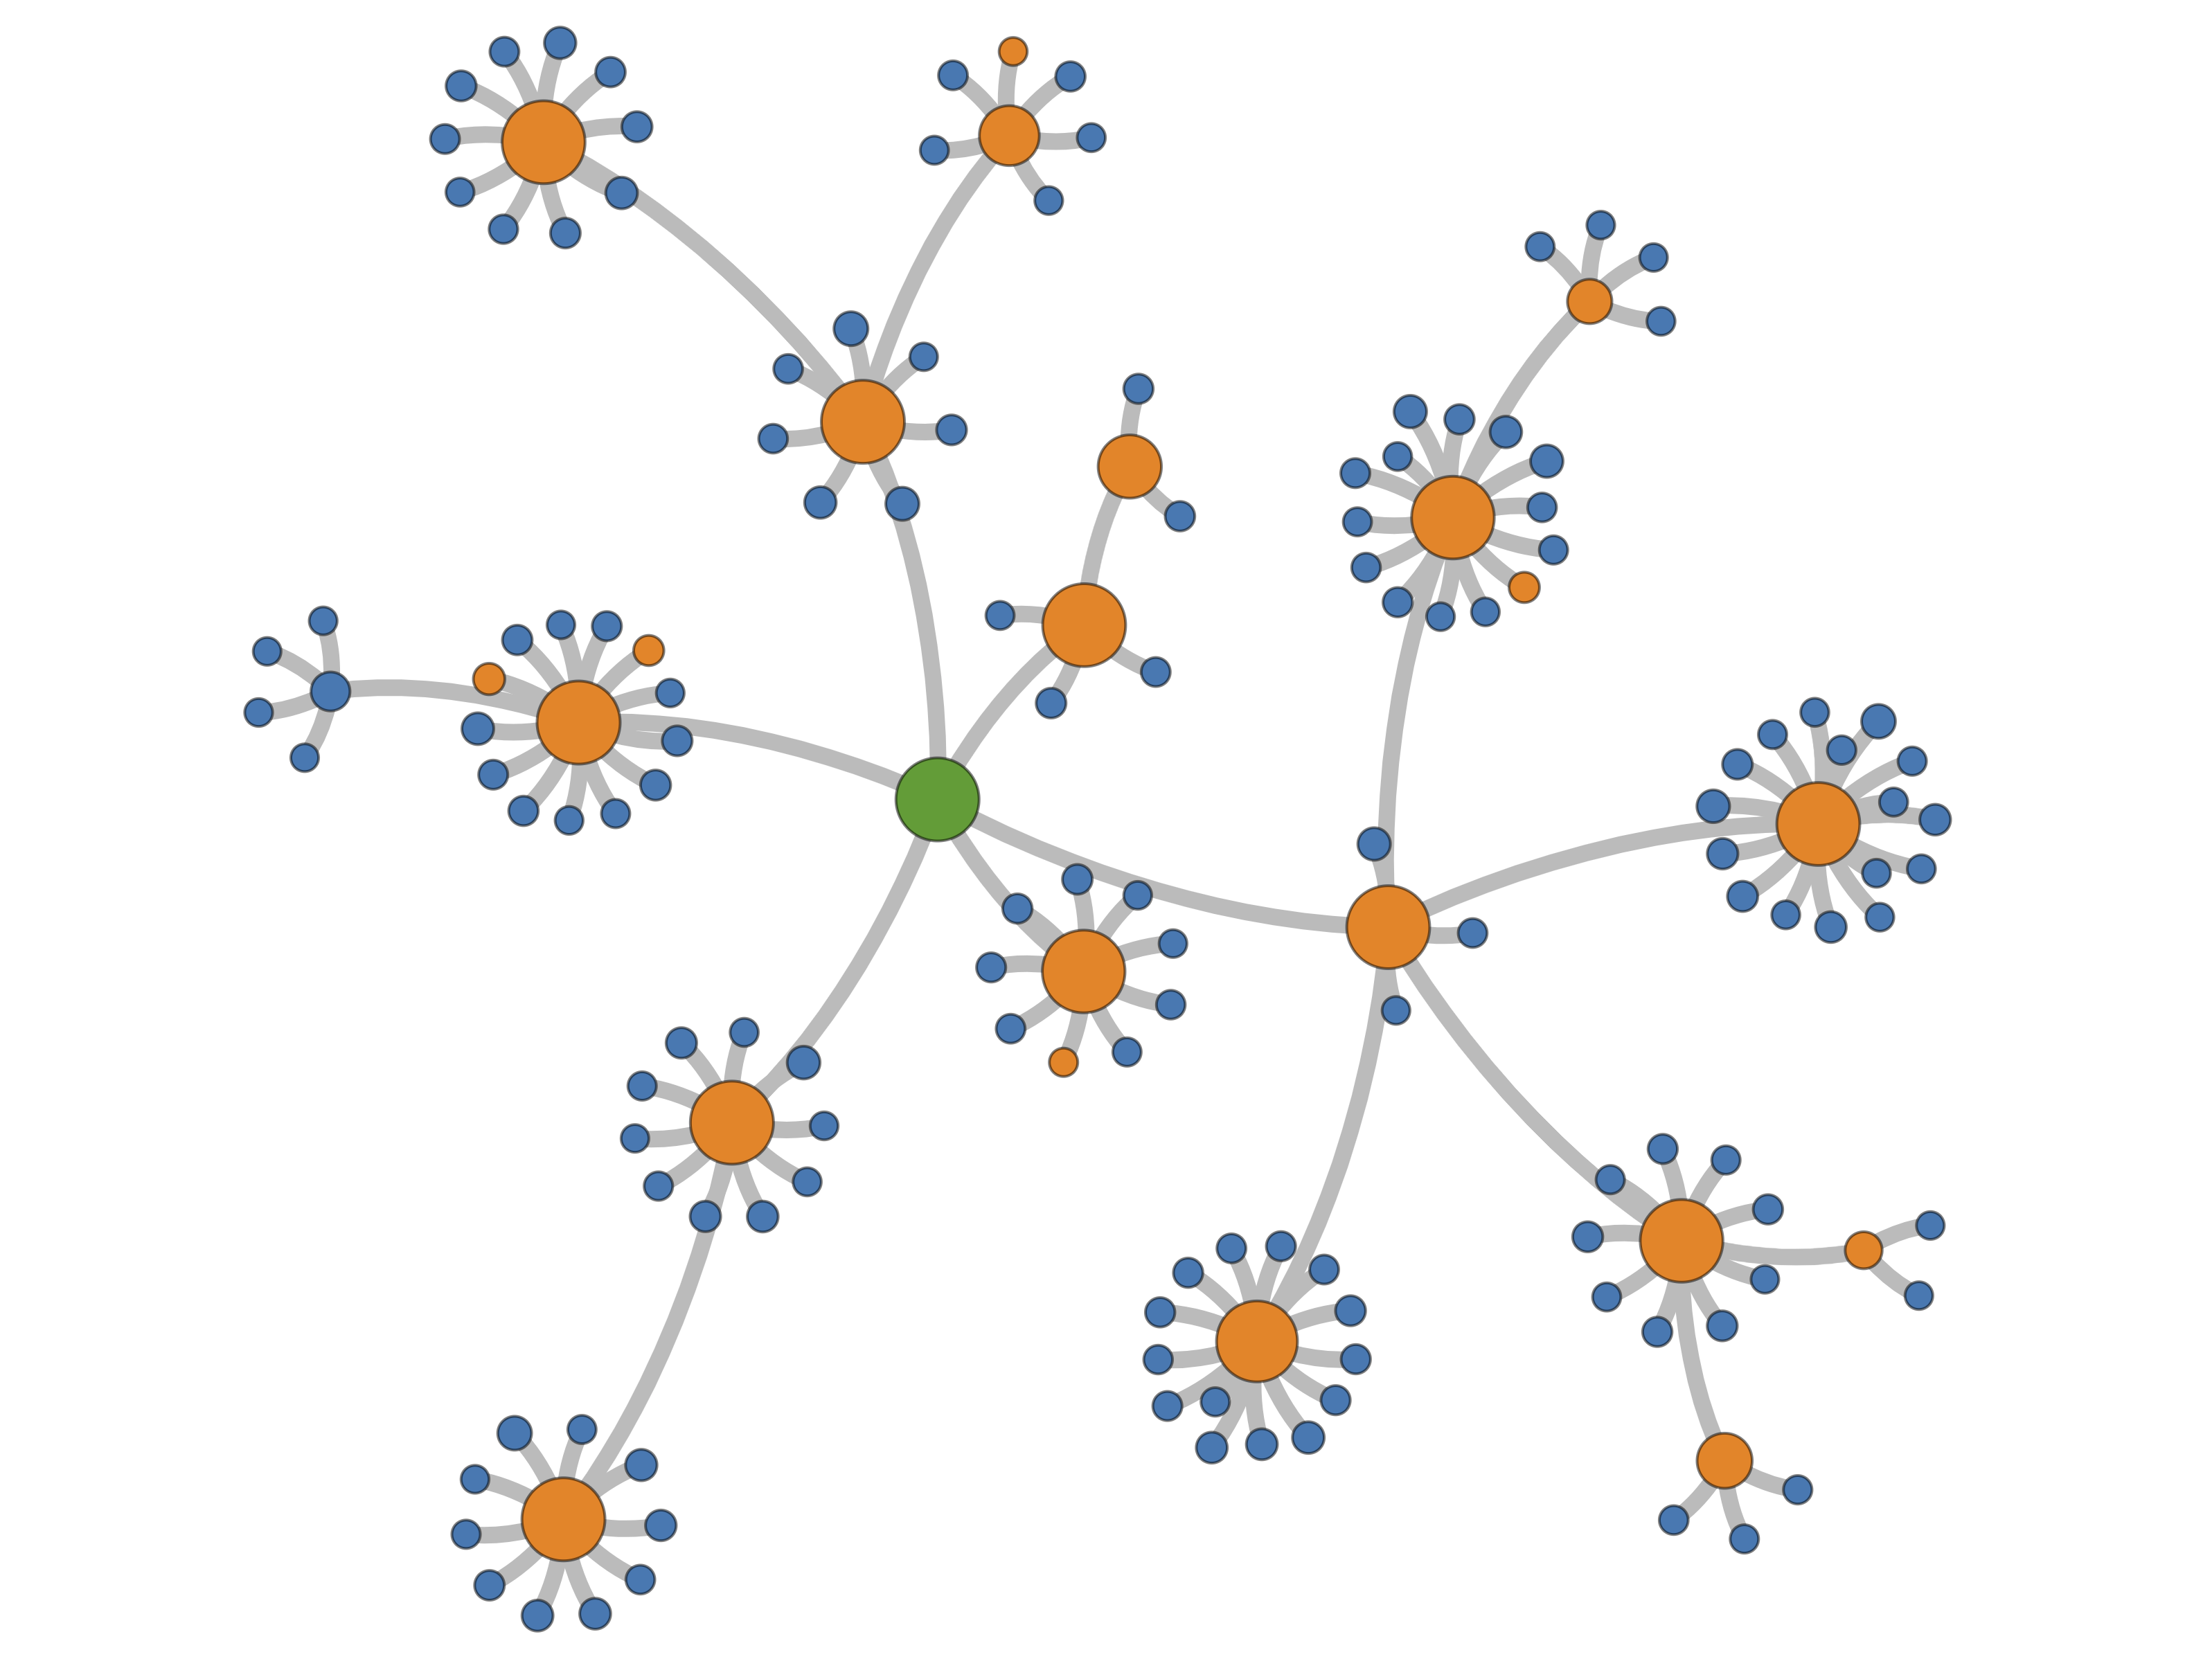
\includegraphics[width=0.85\textwidth]{figures/synthetic 1}
  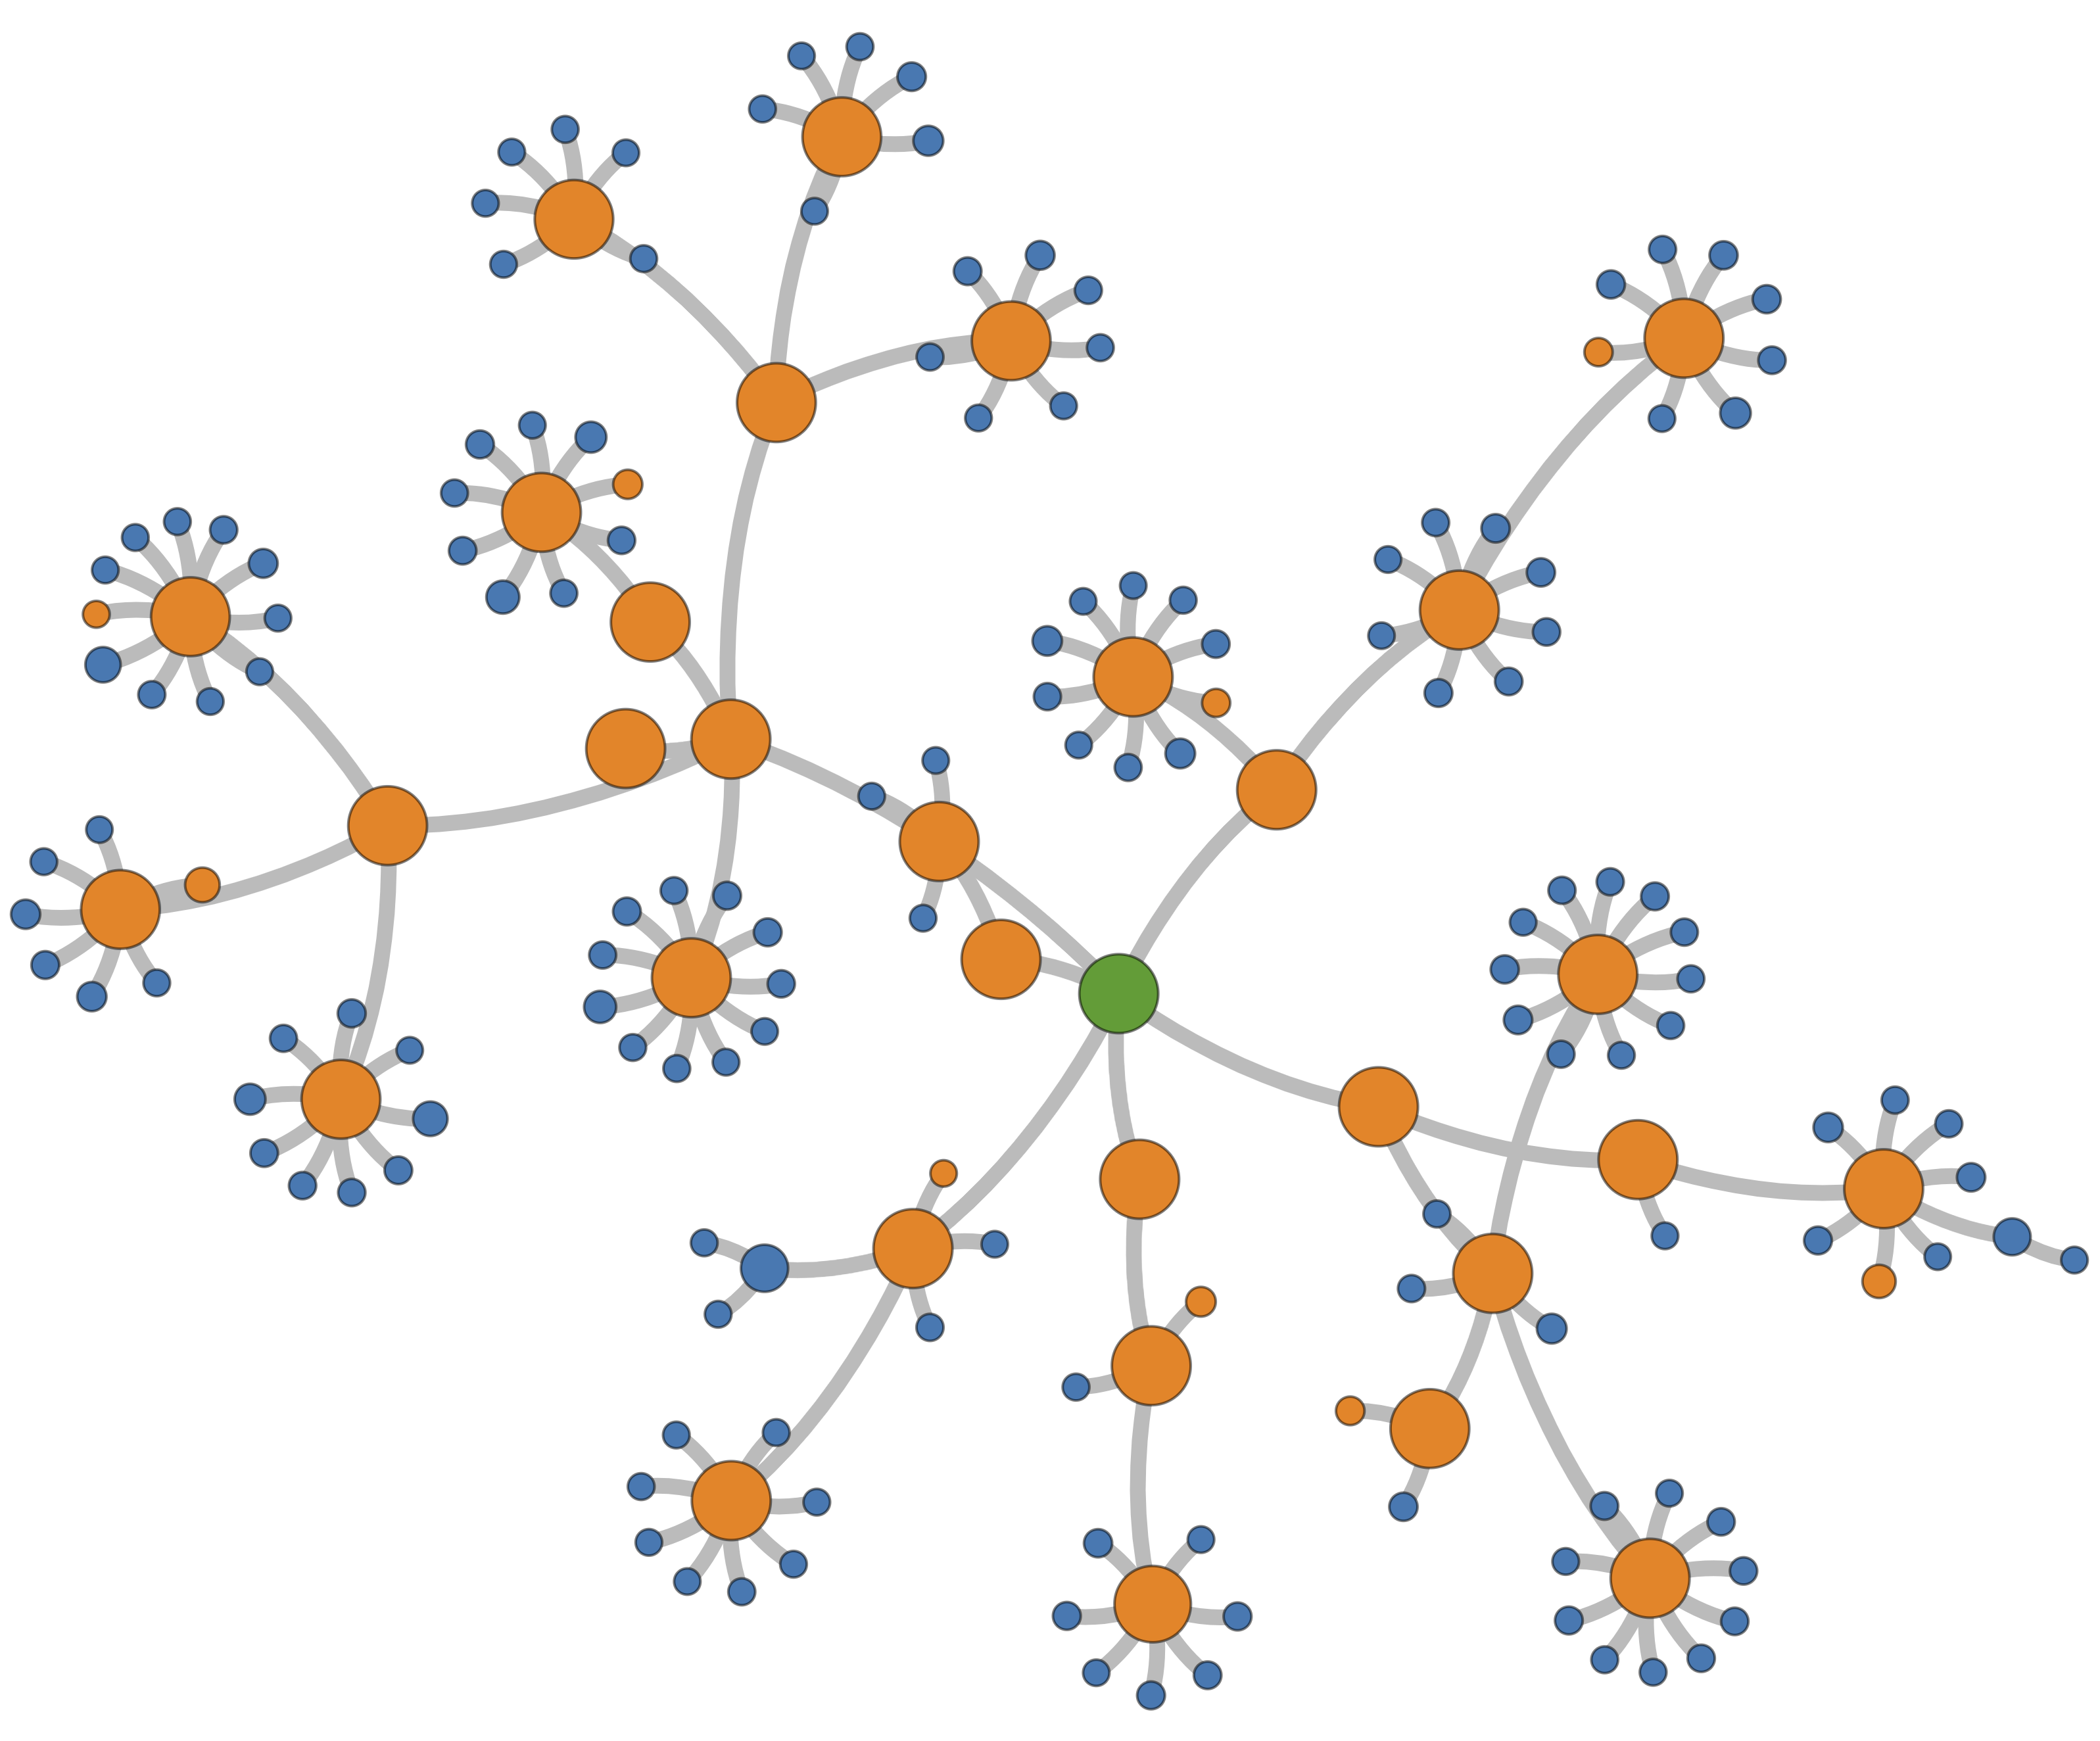
\includegraphics[width=0.85\textwidth]{figures/synthetic 2}
\caption{State trees inferred from synthetic data sequences of 10\,000 (top) and
  1\,000\,000 characters (bottom). The sequences were generated using a single,
  random, 50-state model with a 25-symbol alphabet. States that are present in
  the underlying model are coloured orange, and the root state~\(\lambda\) is
  coloured green.}
\label{fig:25-character model}
\end{figure}

\subsection{Text data}\label{sec:text} %========================================

In this and the next two sections we look for dependencies between symbols in
real-world data sets. We should, however, preface these sections by saying that
it is unlikely that any of the inferences made here will be particularly
enlightening. More realistically, one can expect to gain an understanding of the
way that the length and complexity of a data set influences the marginal state
probabilities estimated by the MCMC procedure, and therefore the state tree
constructed from these probabilities.

We begin by considering two English text data sets: John Keats's \textit{Ode on
Melancholy}, and Charles Dickens's \textit{David Copperfield}. Before any
inference could be performed on these data sets, a few preprocessing steps were
applied: characters were converted to lower case, punctuation marks other than
those that appear within words---such as apostrophes and hyphens---were removed,
and all whitespace characters were treated identically.

We consider two straightforward ways of viewing bodies of text as sequences: by
treating either characters or words as symbols. In the former case the symbol
alphabets for the two documents are of sizes~26 and~41 (for Keats and Dickens
respectively), and the lengths of the data sets are~1\,223 and~1\,843\,427. When
considering \emph{words} as symbols, the alphabets contain~157 and~15\,289
symbols respectively, and the sequences are of lengths~223 and~357\,043. We note
here though that in the per-word case, we used a subset of the Dickens document
consisting of the first ten chapters (5\,724 unique symbols; sequence-length
54\,961) for performance reasons. Marginal probabilities for both data sets were
estimated based on 100\,000 sampled models, and trees were again constructed
using those states whose probabilities were greater than or equal to~0.1.

Inference results for Keats's \textit{Ode on Melancholy} are given in
Table~\ref{tab:text 1} and Figure~\ref{fig:text 1}. As was the case for the
largest of the synthetic data sets, a full description of the results is not
possible here. As such, the table contains a few of the highest-probability
states from the MCMC simulation, and the figure provides an overview of the
marginal probabilities by means of a reconstructed state tree.
%
\begin{table}[htbp]
\centering
\begin{tabular}{llccllc}
  \toprule
  \multicolumn{3}{c}{Characters} && \multicolumn{3}{c}{Words} \\
  \cmidrule{1-3} \cmidrule{5-7}
  \(s\) & \(\hat{\Pb}(s)\) & \(\argmax_x \ub{n}_s(x)\) &&
  \(s\) & \(\hat{\Pb}(s)\) & \(\argmax_x \ub{n}_s(x)\) \\
  \midrule
  a  & 1.0   & n: 18    && \(\lambda\) & 1.0   & the: 14, \dots \\
  c  & 0.308 & h: 5     && and         & 0.739 & be: 1, let: 1, \dots \\
  ee & 0.960 & p: 3     && her         & 0.870 & soft: 1, rave: 1, \dots \\
  ie & 0.106 & s: 4     && rich        & 0.102 & anger: 1 \\
  an & 0.508 & d: 10    && soul        & 0.209 & but: 1, shalt: 1 \\
  o  & 1.0   & r, u: 13 && that        & 0.206 & fosters: 1, must: 1 \\
  jo & 0.426 & y: 2     && the         & 0.999 & beetle: 1, death-moth: 1, \dots \\
  t  & 0.916 & h: 28    && thy         & 0.368 & pale: 1, sorrow: 1, mistress: 1 \\
  \bottomrule
\end{tabular}
\caption{Example state probabilities derived from Keats's \textit{Ode on
  Melancholy}, when treated as a sequence of characters and words respectively.}
\label{tab:text 1}
\end{table}
%
\begin{figure}[htbp]
\centering
  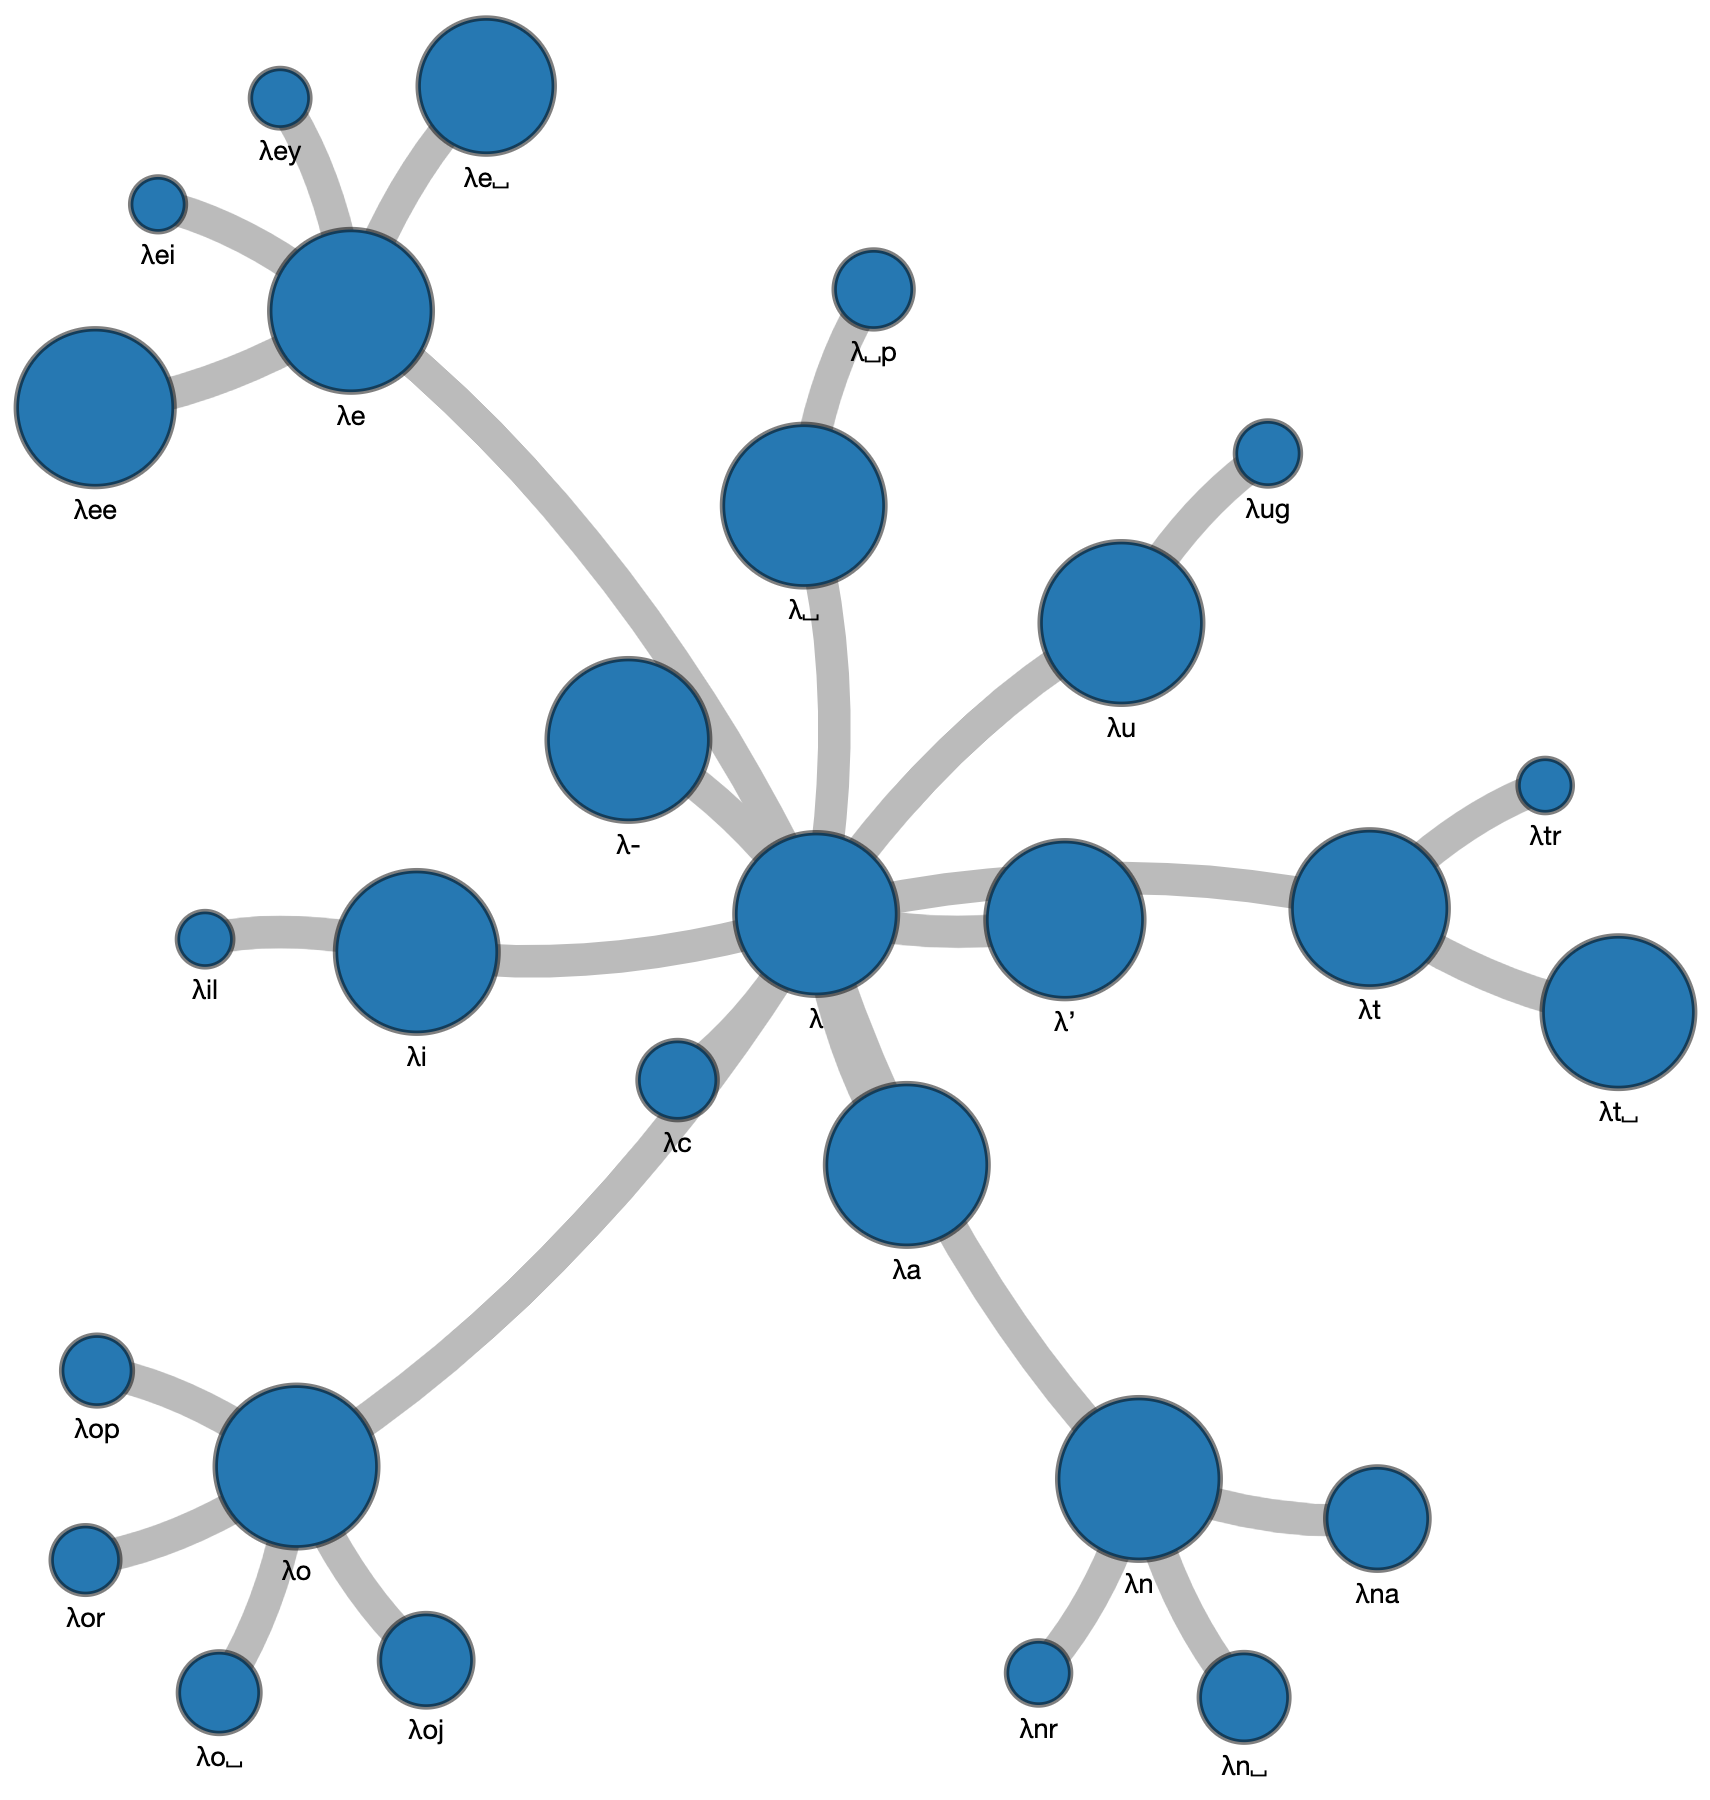
\includegraphics[width=0.7\textwidth]{figures/text 1c} \\
  \vspace{1em}
  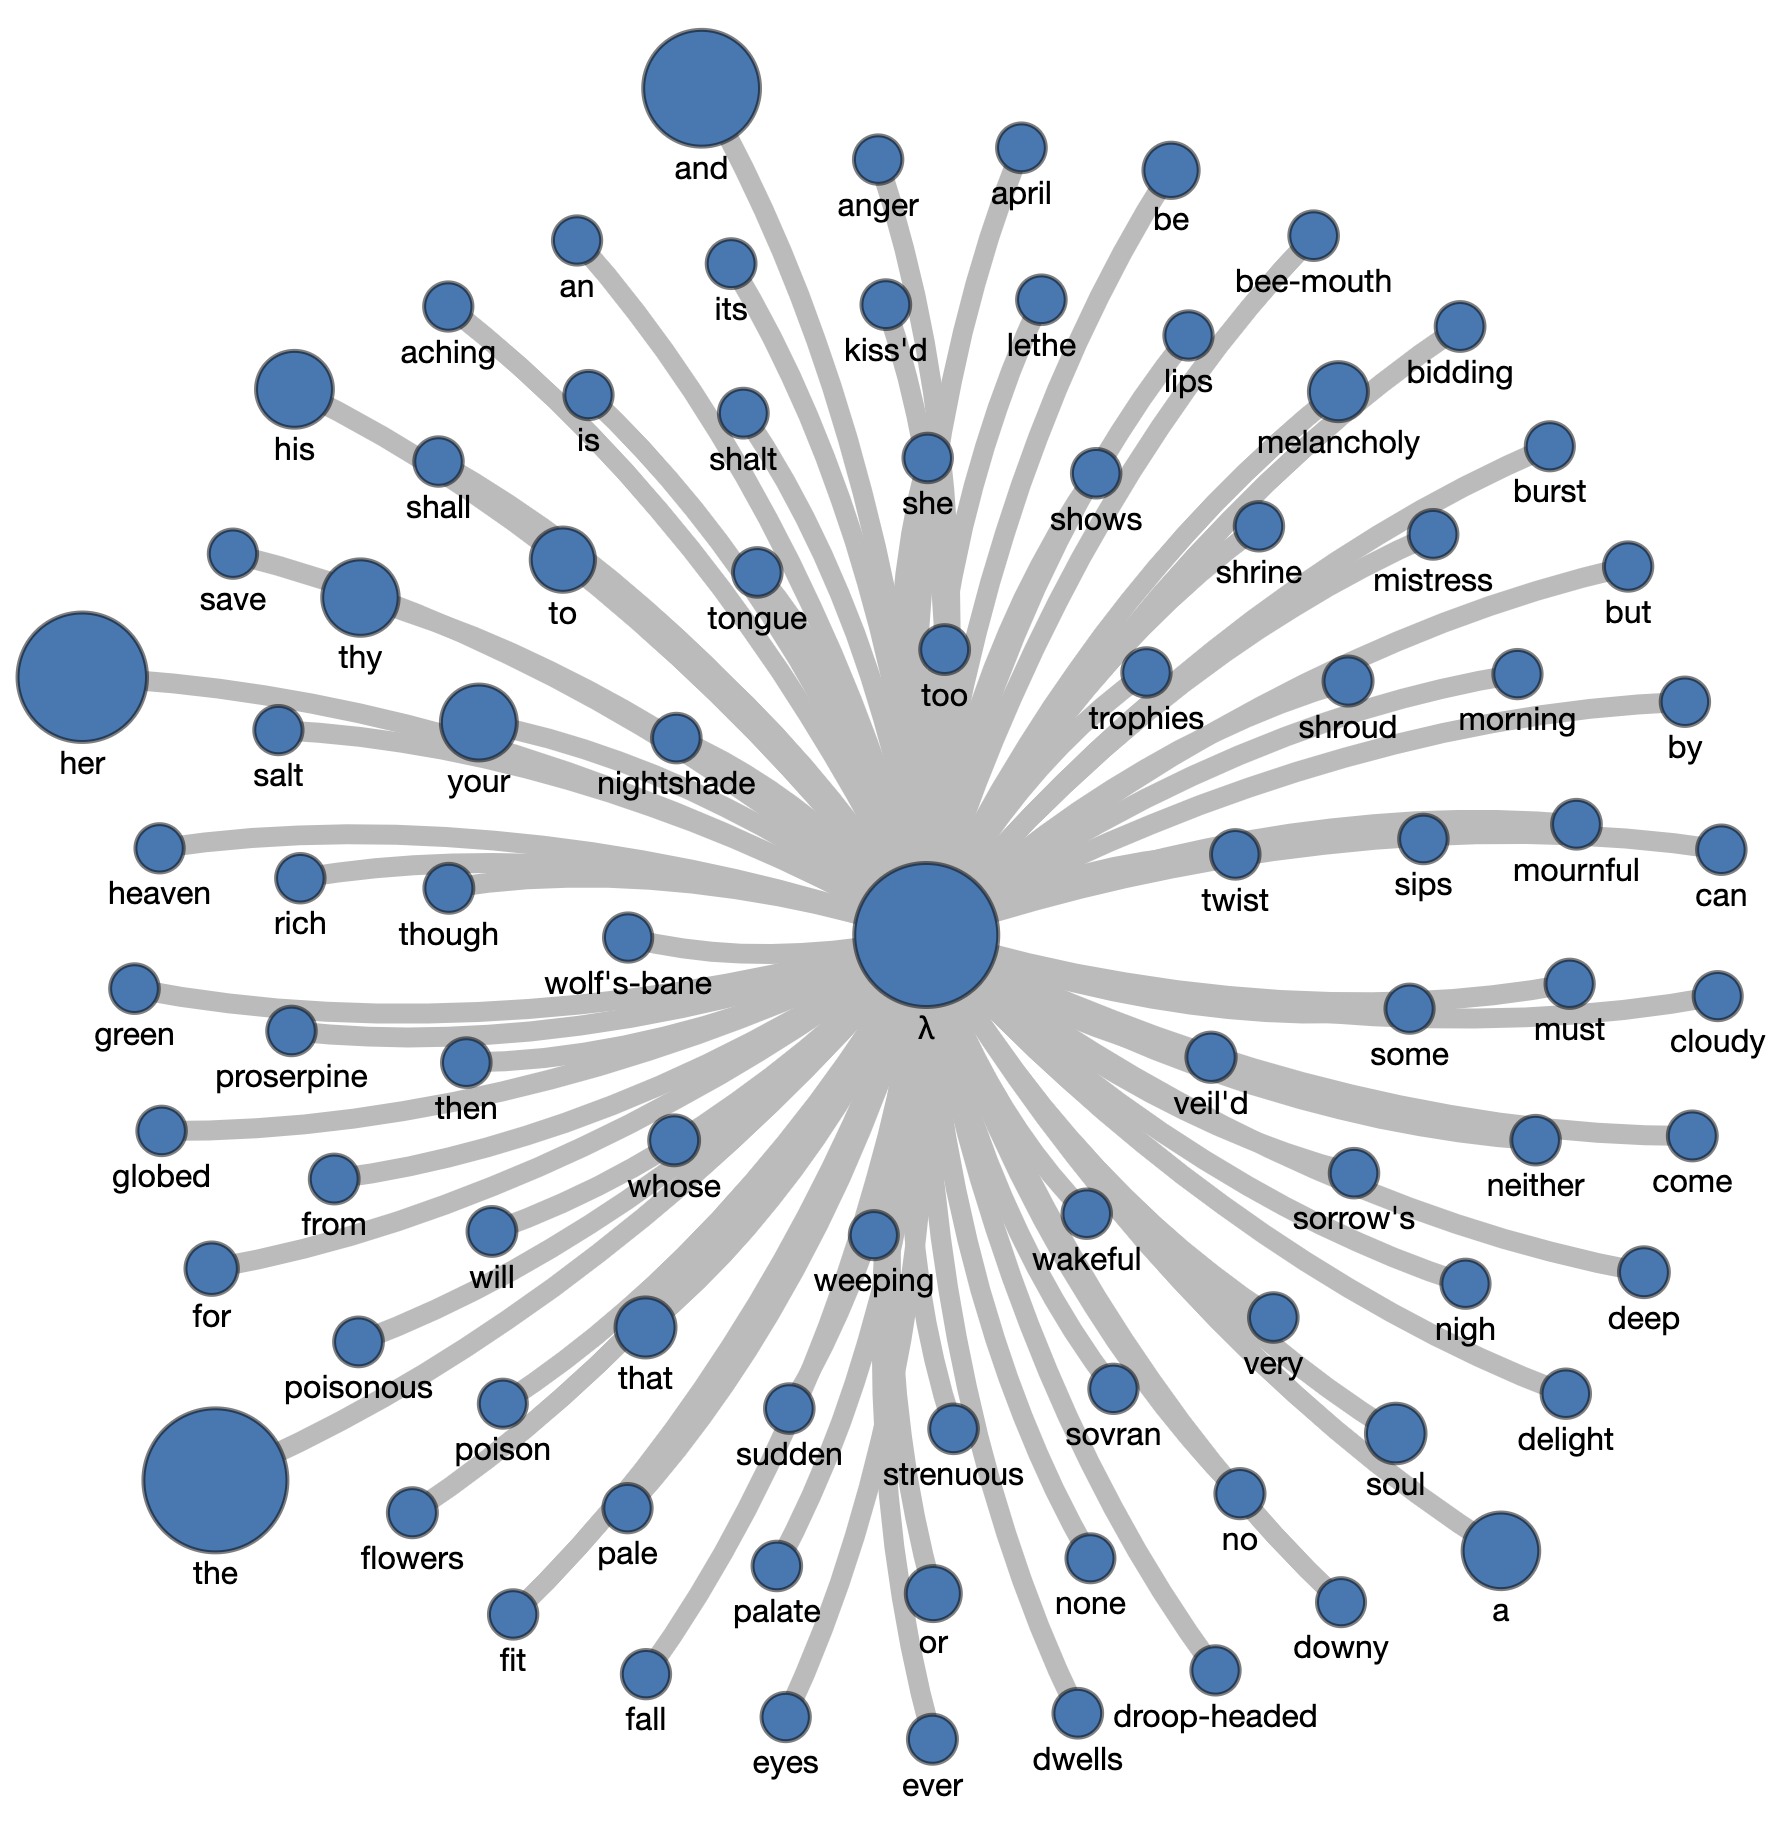
\includegraphics[width=0.7\textwidth]{figures/text 1w}
\caption{Approximate marginal state probabilities inferred from the poem
  \textit{Ode on Melancholy} by John Keats, treating individual characters (top)
  and entire words (bottom) as symbols respectively.}
\label{fig:text 1}
\end{figure}

One sees from the table, for example, that the prefix~`jo' is present in the
Keats tree due to its two occurrences as part of the word `joy'. The figures, on
the other hand, show the effect that an increased alphabet size has on the
inference procedure: there is now far less data to support each symbol
state---and even less to support longer, compound states.

Notice that only three of the words present in the Keats poem have estimated
probabilities greater than~0.5:~`and', `her', and~`the'. It is perhaps
interesting to see that these states have been assigned high probabilities even
though their empirical distributions are relatively flat (consisting of sets of
words that each only appear once); but these distributions are of course
significantly different to that of the root state~\(\lambda\), whose most likely
elements are~`the'~(14 occurrences), `of'~(8), `and`~(7), and~`her'~(6).

The results for Dickens's \textit{David Copperfield} are presented in
Table~\ref{tab:text 2} and Figure~\ref{fig:text 2c}, and they are understandably
very different from those of the smaller data set. The length of the data
provides far more support for specific character sequences; for example `mf'
(not shown in the table below) is considered a significant prefix in the Dickens
book because it is almost followed by the symbol~`o'---as in the word~`comfort'
and its various derivatives.
%
\begin{table}[htbp]
\centering
\begin{tabular}{llccllc}
  \toprule
  \multicolumn{3}{c}{Characters} && \multicolumn{3}{c}{Words} \\
  \cmidrule{1-3} \cmidrule{5-7}
  \(s\) & \(\hat{\Pb}(s)\) & \(\argmax_x \ub{n}_s(x)\) &&
  \(s\) & \(\hat{\Pb}(s)\) & \(\argmax_x \ub{n}_s(x)\) \\
  \midrule
  rie   & 0.942 & d: 478, n: 408, \dots && mr      & 0.985 & creakle: 69, \dots \\
  arie  & 0.914 & t: 24, s: 9, \dots    && my      & 0.994 & mother: 224, \dots \\
  prie  & 0.838 & t: 6                  && shadowy & 0.188 & world: 2, \dots \\
  erie  & 0.921 & n: 55, s: 18, \dots   && dutch   & 0.495 & clock: 3 \\
  perie & 0.889 & n: 55, \dots          && young   & 1.0   & copperfield: 8, \dots \\
  frie  & 0.930 & n: 353, d: 1          && i       & 0.973 & was: 188, had: 132, \dots \\
  brie  & 0.832 & f: 8                  && little  & 0.980 & em’ly: 25, \dots \\
  hrie  & 0.940 & k: 5                  && some    & 0.979 & of: 14, time: 9, \dots \\
  grie  & 0.914 & f: 30, v: 11          && rat     & 0.978 & tat-tat: 9 \\
  \bottomrule
\end{tabular}
\caption{Example state probabilities derived from Dickens's \textit{David
  Copperfield}, when treated as a sequence of characters and words respectively.}
\label{tab:text 2}
\end{table}
%
\begin{figure}[htbp]
\centering
  \makebox[\textwidth][c]{
    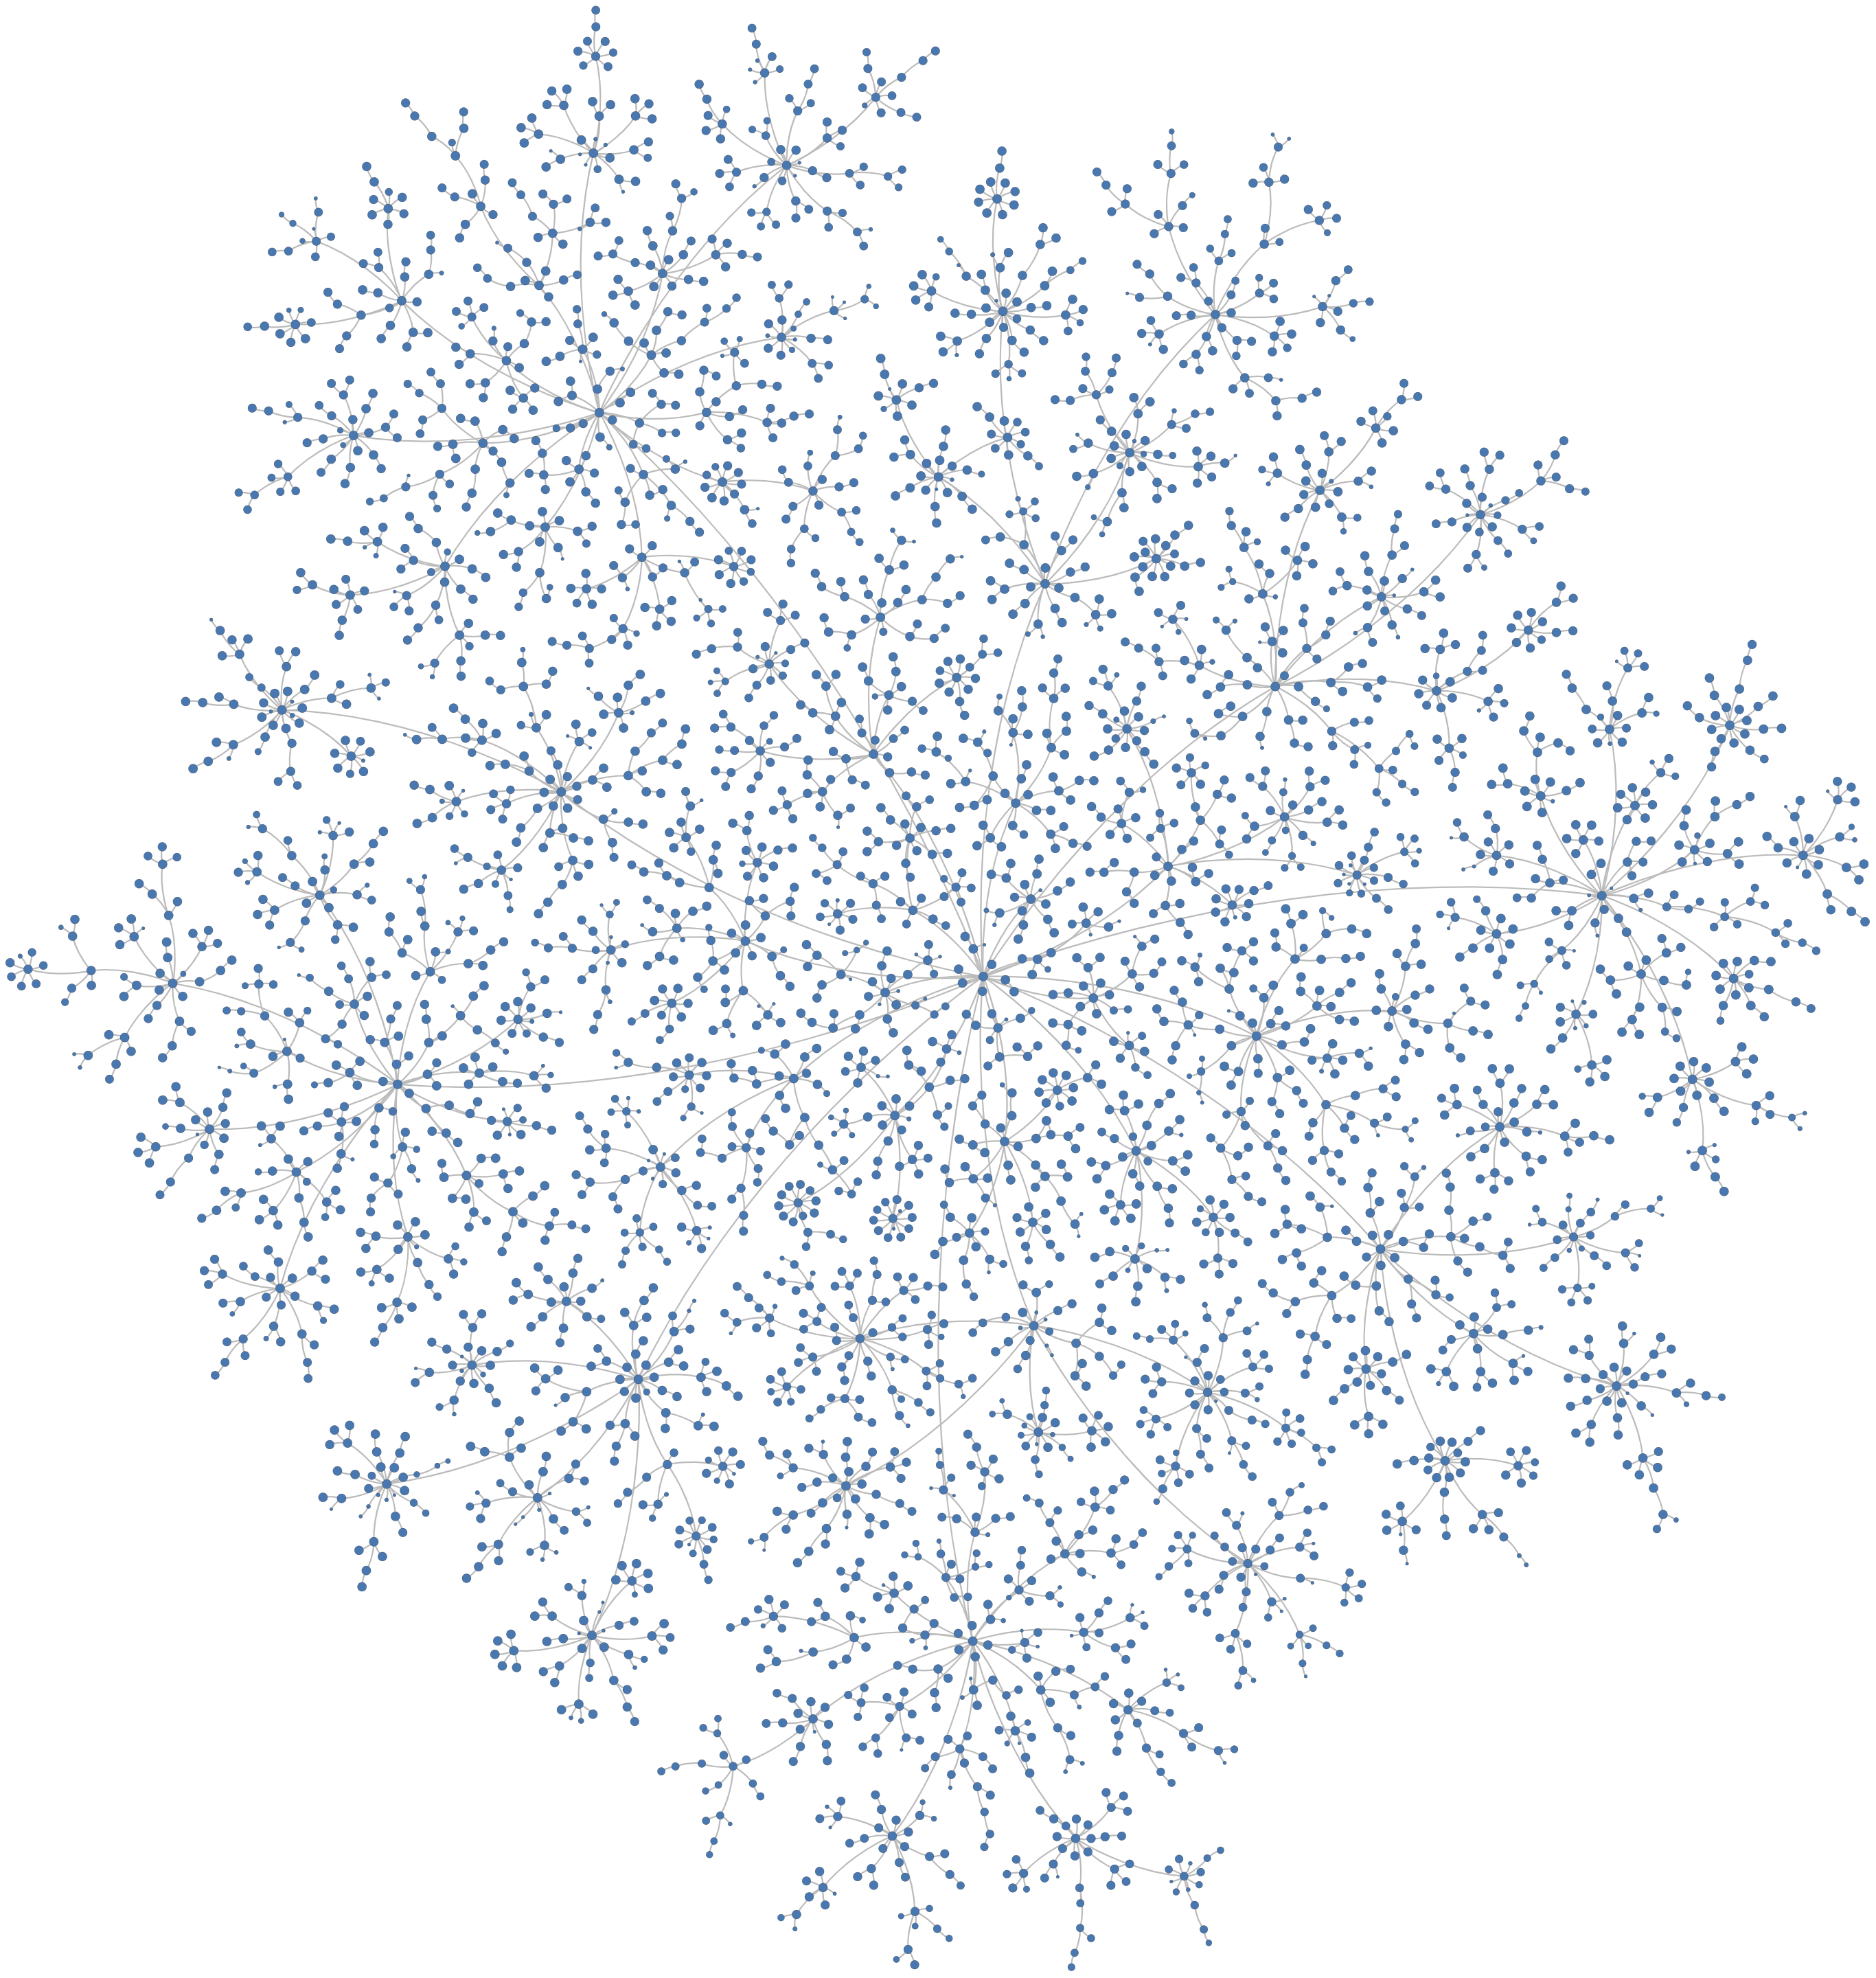
\includegraphics[width=1.25\textwidth]{figures/text 2c}
  }
\caption{The state tree constructed from approximate marginal state
  probabilities inferred from \textit{David Copperfield} by Charles Dickens,
  treating individual characters as symbols.}
\label{fig:text 2c}
\end{figure}

The sheer number of such states is quite impressive: Figure~\ref{fig:text 2c},
containing all of the states whose probabilities exceed 0.1, is made up of
4\,280 nodes. The examples given in the left column of Table~\ref{tab:text 2}
were simply chosen from one of the small, fringe subtrees present in the figure
(the most `northerly' star, from which two nodes extend upwards, if the reader
is particularly curious).

When it comes considering whole words as symbols, the comments made regarding
the Keats poem are even more applicable in the case of the Dickens book: only a
relatively small subset of single-word states are assigned high probabilities.
Although we do not include them in a figure here, a few examples are given in
the right column of Table~\ref{tab:text 2}.

\subsection{Temporal networks}\label{sec:temporal networks} %===================

The variable-order Markov models described here can also be applied to forms of
data that differ slightly from the more typical sequences dealt with above---as
long as Markov states can be associated with each symbol in the data set. In
this section we consider temporal network (or graph) data, which are
\emph{ordered} sequences of source-destination pairs~\(\ub{x} = (v_1, w_1),
(v_2, w_2), \dots\) in which the~\(v_i\) and~\(w_i\) are both elements of a node
set~\(\mc{A}\).

We are interested in directed, temporal paths made up of edges in the network,
which will appear as non-consecutive pairs in the data set; for example:
\((v_{i_1}, w_{i_1}), (v_{i_2} \peq w_{i_1}, w_{i_2}), (v_{i_3} \peq w_{i_w},
w_{i_3}), \dots\). Notice how every node along a path (apart from the initial
source and final destination) appears twice---first as a destination and second
as a source.

It will prove convenient to treat source nodes~\(v_i\) as states and
destinations~\(w_i\) as symbols. To construct a prefix for an observed
symbol~\(w_n\), one simply needs to follow the path of edges that terminates
at~\(w_n\) in reverse, considering states along the way. Adopting the indices of
the previous paragraph, the prefix of length~\(k\) for the symbol~\(w_{i_n}\)
would be~\(v_{i_{n-k+1}}, \dots, v_{i_{n-1}}, v_{i_n}\).

Apart from this artificial separation between states and symbols, temporal
networks can be treated in much the same way as straightforward
sequences.\footnote{Note however that we have not placed any restrictions on the
edge paths that result in prefixes here. One could, for example, take timestamps
into account and require that an incoming edge occur within a certain amount of
time of the following outgoing edge for its source to be considered as the next
possible state in the prefix.} We have treated two temporal networks here: one
derived from emails sent within a research institution~\cite{snapnets}, and the
other from phone calls made between participants of a social network
study~\cite{aharony2011social}. The email network contains 89 nodes (i.e.,
unique symbols) and 12\,216 timestamped edges, and the call dataset consists of
122 nodes and 164\,906 edges.

Inferred probabilities for the two networks are shown as state trees in
Figure~\ref{fig:network}. One sees that the vast majority of prefixes are simply
first-order Markov states, which implies that nodes in the network have their
own outgoing probability distributions (as opposed to a global distribution over
edge destinations). In a few cases, second-order states are also present: these
almost always correspond to reciprocal communication, i.e., edge sequences of
the form~\((v_j, v_i)), (v_i, v_j)\). We have also included a sample of states
from each data set in Table~\ref{tab:network}, where one can see the most likely
destinations conditioned on each state. Perhaps weaker model priors---or simply
larger or richer data sets---are required if we are to obtain more complex
marginal state trees.
%
\begin{figure}[htbp]
\centering
  \makebox[\textwidth][c]{
    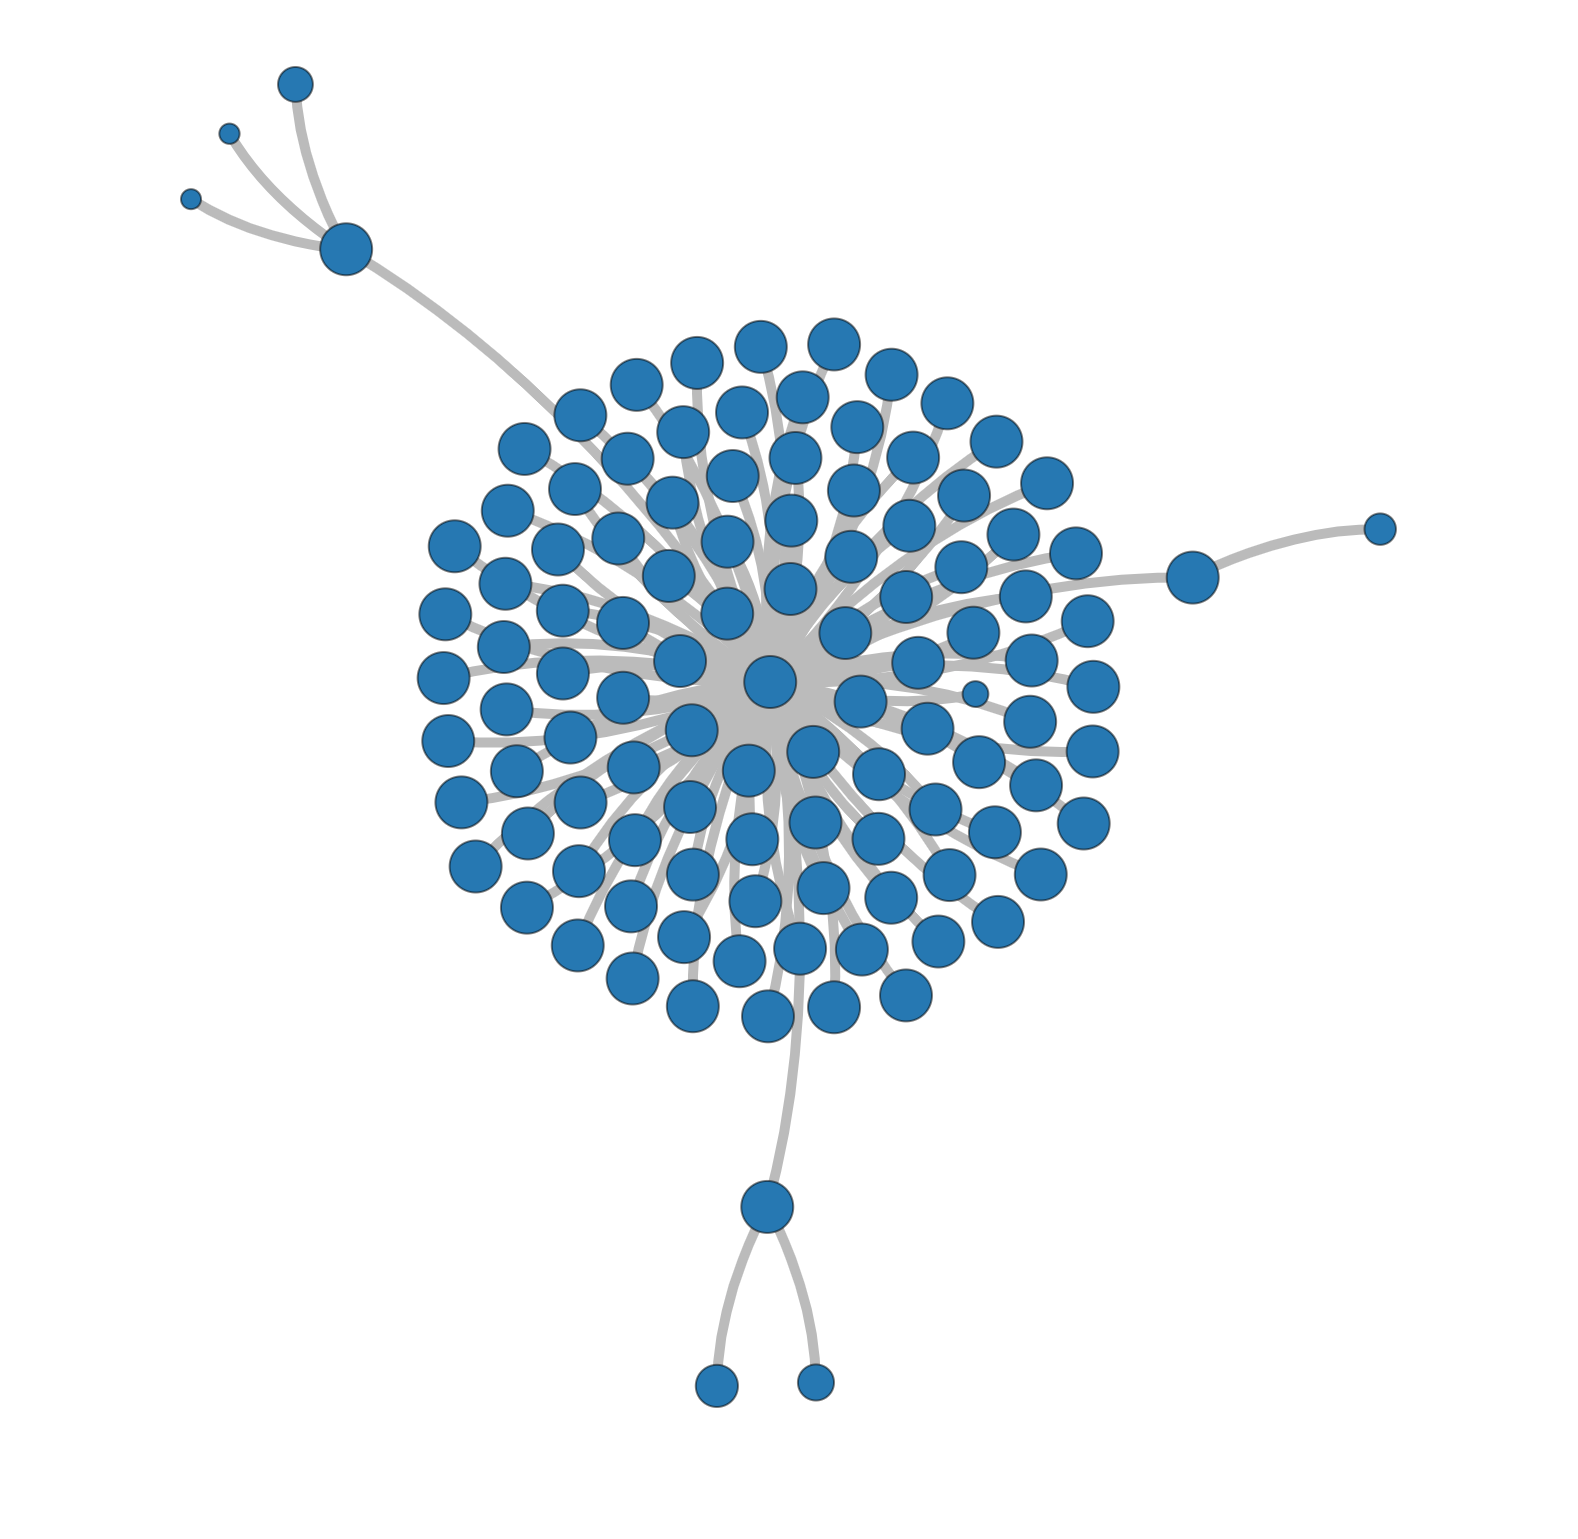
\includegraphics[width=0.5\textwidth]{figures/network 1}
    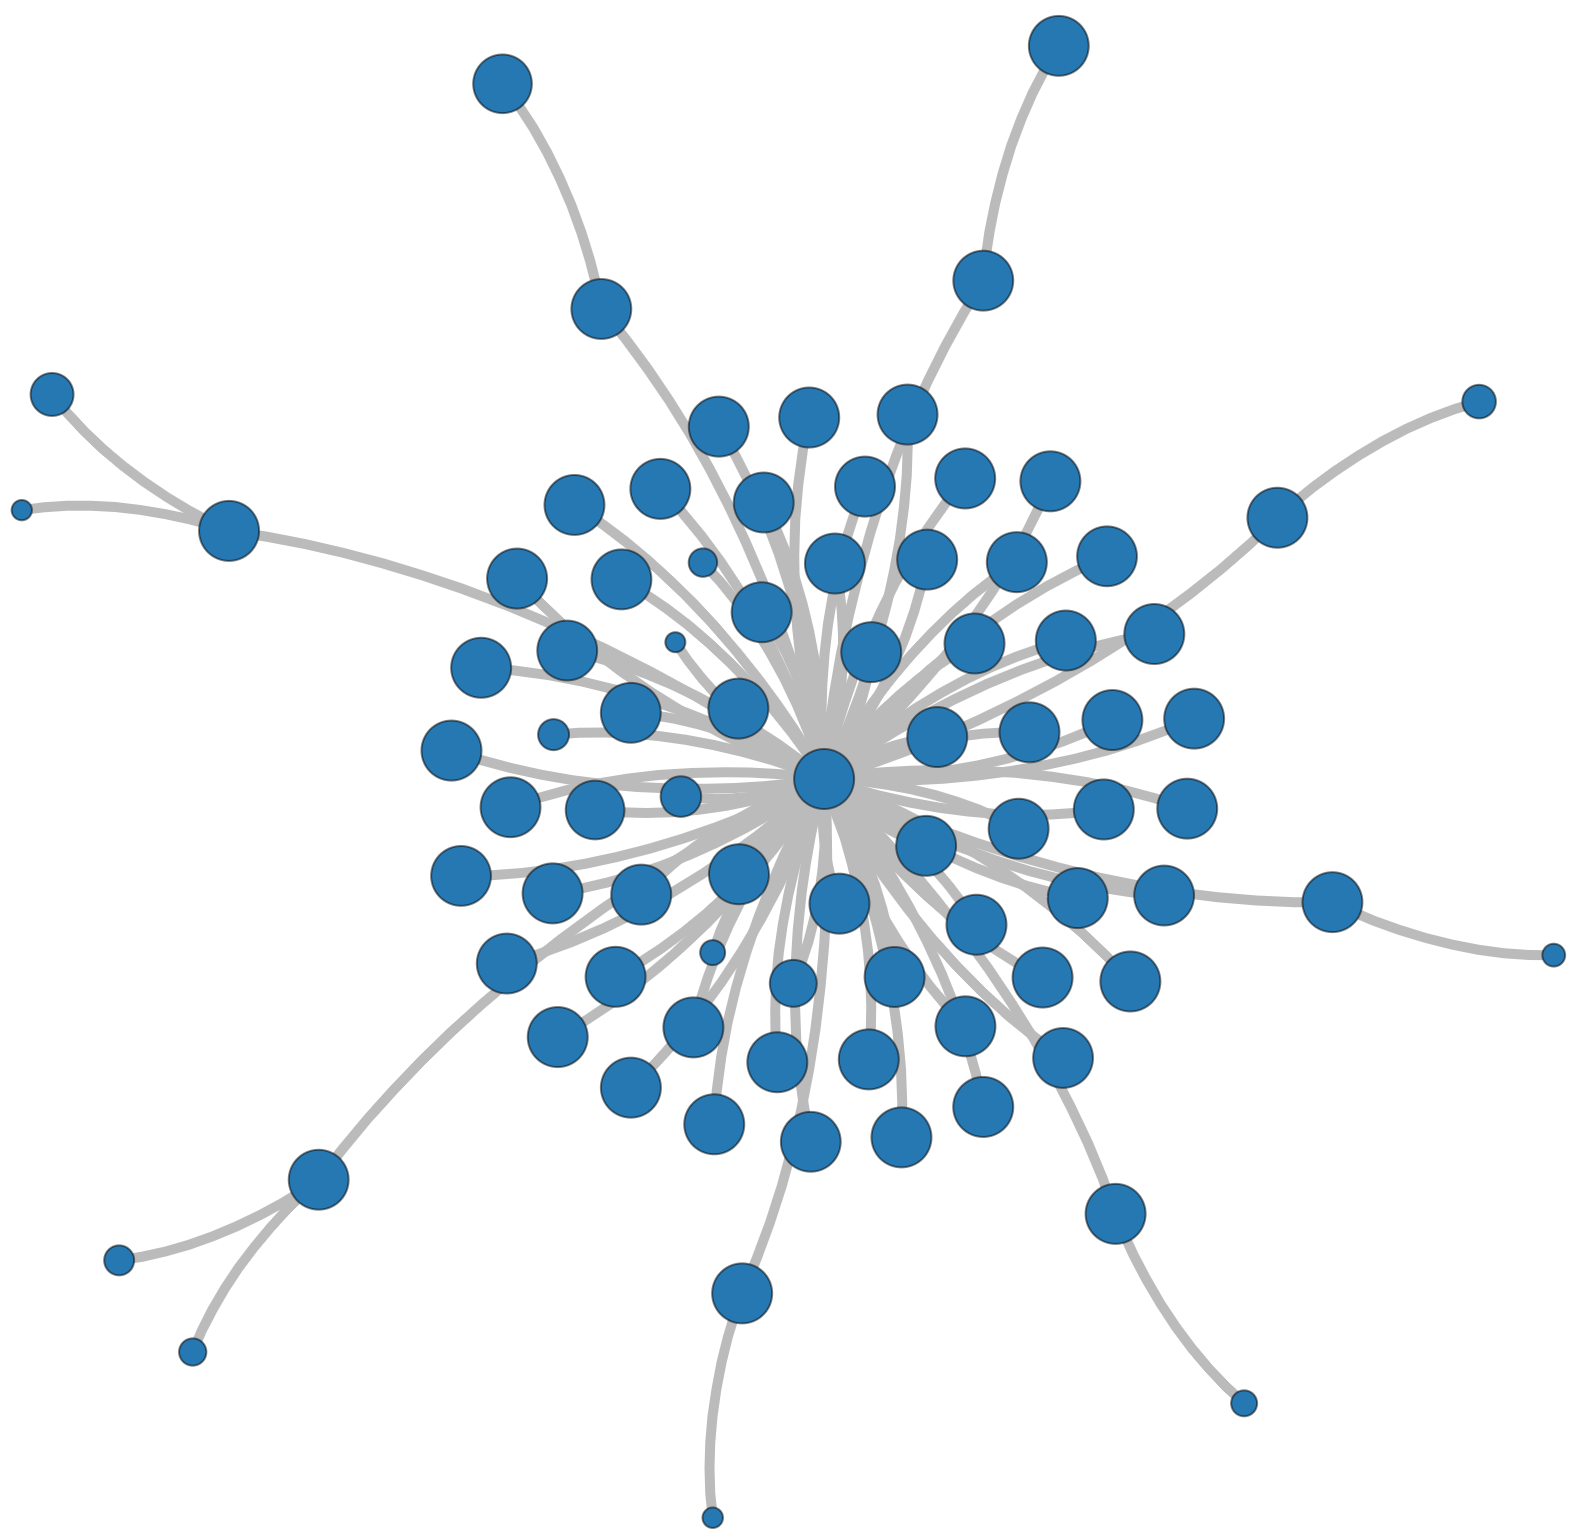
\includegraphics[width=0.5\textwidth]{figures/network 2}
  }
\caption{Marginal state probabilities based on two temporal network data sets:
  one consisting of call metadata (left), the other of email metadata (right).}
\label{fig:network}
\end{figure}
%
\begin{table}[htbp]
\centering
\begin{tabular}{llccllc}
  \toprule
  \multicolumn{3}{c}{Calls} && \multicolumn{3}{c}{Emails} \\
  \cmidrule{1-3} \cmidrule{5-7}
  \(s\) & \(\hat{\Pb}(s)\) & \(\argmax_x \ub{n}_s(x)\) &&
  \(s\) & \(\hat{\Pb}(s)\) & \(\argmax_x \ub{n}_s(x)\) \\
  \midrule
  \(\lambda\) & 1.0   & f13: 1895, f21: 1205, \dots && \(\lambda\) & 1.0 & 54: 615, \dots \\
  f44         & 1.0   & f43: 625, \dots             && 49          & 0.998 & 54: 106, \dots \\
  f43         & 1.0   & f44: 240, \dots             && 35-49       & 0.382 & 35: 3, 15: 3, \dots \\
  f64         & 0.998 & f63: 422, f64: 4            && 23-49       & 0.273 & 54: 2, 60: 1, \dots \\
  f63         & 0.999 & f64: 430, f63: 7, \dots     && 47          & 0.924 & 23: 4, \dots \\
  f53-f82     & 0.571 & s53: 4                      && 74          & 0.727 & 35: 4, \dots \\
  f43-f82     & 0.134 & f43: 3                      && 42          & 1.000 & 45: 27, \dots \\
  s71-f82     & 0.133 & f71: 3                      && 45          & 0.997 & 42: 20, \dots \\
  \bottomrule
\end{tabular}
\caption{Example state probabilities inferred from a pair of temporal network
  data sets.}
\label{tab:network}
\end{table}

% \subsection{Genetic data}\label{sec:genetic} %==================================

\subsection{Unstructured data}\label{sec:unstructured} %========================

A final simple, but nonetheless interesting test of our inference approach is to
apply it to unstructured data. In particular, we consider data generated
according to a single categorical distribution (i.e., using the trivial,
single-state model~\(\mc{S} = \{\lambda\}\)), and investigate the rate at which
the marginal probabilities of the non-trivial states converge to zero.

Recall that the state probabilities estimated by an MCMC simulation are always
non-decreasing along paths away from the root (e.g., \(\Pb(bc) \le \Pb(c) \le
\Pb(\lambda)\)), so we only need consider the probabilities assigned to the
root's direct children to obtain the maximum marginal probability over all
non-root states. We measure the rate at which this maximum decreases over data
sets that range in length from~10 to~10\,000 symbols, for three different
models.

The three models we consider have symbol alphabets of sizes~2, 10, and~20, and
as mentioned above, consits only of the root state~\(\lambda\). In the binary
case we consider two categorical distributions: the uniform distribution~\(\Pb(x
\peq 1) = 0.5\) as well as another distribution chosen randomly. Since there is
no significant difference between the results for these two binary
distributions, we only consider uniform distributions when dealing with the 10-
and 20-character models. Note that in the binary case, the model space was
restricted to that of \emph{full} binary trees, implying that the marginal
probabilities of the root's children were always equal: \(\hat{\Pb}(0) =
\hat{\Pb}(1)\).

Figure~\ref{fig:unstructured} shows the consolidated results for the three
models. For each model and each sequence length~\(\abs{\ub{x}}\), we
generated~20 random sequences according to the model's categorical distribution
and measured the maximum (non-root) marginal probability for each; the medians
and quartiles of these measurements were used to plot the traces in the figure.
Each MCMC simulation was run until 10\,000 samples had been drawn.
%
\begin{figure}[htbp]
\centering
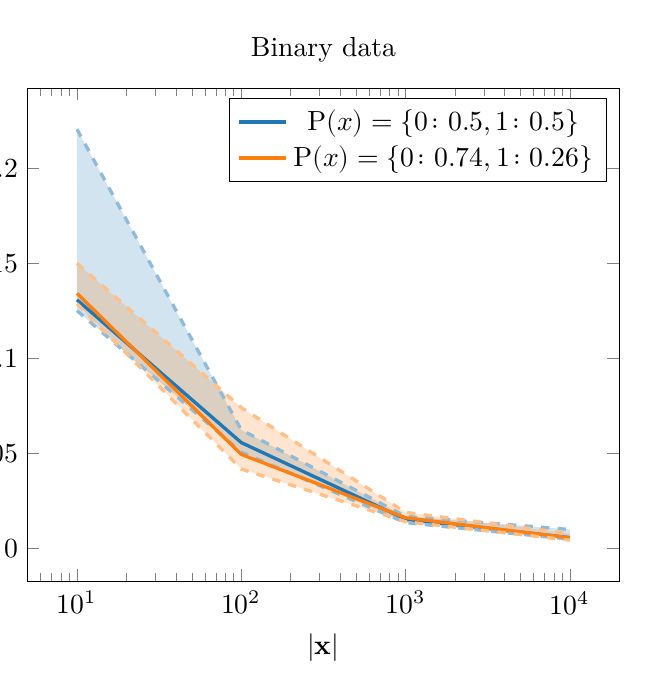
\begin{tikzpicture}[trim axis left, trim axis right]
\begin{semilogxaxis}[
  title={Binary data},
  xlabel=\(\abs{\ub{x}}\),
  ylabel=\(\ds \max_{s\ne\lambda} \Pb(s)\),
  yticklabel style={/pgf/number format/fixed},
  legend entries={
    {\(\Pb(x) = \{0\colon 0.5, 1\colon 0.5\}\)},
    {\(\Pb(x) = \{0\colon 0.74, 1\colon 0.26\}\)}
  }
]
  \addplot[cbblue,name path=median 1]
    coordinates{(10, 0.1308) (100, 0.0557) (1000, 0.0154) (10000, 0.0057)};
  \addplot[cbblue!50,dashed,name path=lower 1,forget plot]
    coordinates{(10, 0.1251) (100, 0.0507) (1000, 0.0136) (10000, 0.0049)};
  \addplot[cbblue!50,dashed,name path=upper 1,forget plot]
    coordinates{(10, 0.2205) (100, 0.0624) (1000, 0.0169) (10000, 0.01)};
  \addplot[cbblue,fill opacity=0.2,forget plot]
    fill between[of=lower 1 and upper 1];
  \addplot[cborange,name path=median 2]
    coordinates{(10, 0.1342) (100, 0.0495) (1000, 0.0162) (10000, 0.0056)};
  \addplot[cborange!50,dashed,name path=lower 2,forget plot]
    coordinates{(10, 0.1287) (100, 0.0418) (1000, 0.0141) (10000, 0.0044)};
  \addplot[cborange!50,dashed,name path=upper 2,forget plot]
    coordinates{(10, 0.15) (100, 0.0741) (1000, 0.019) (10000, 0.0078)};
  \addplot[cborange,fill opacity=0.2,forget plot]
    fill between[of=lower 2 and upper 2];
\end{semilogxaxis}
\end{tikzpicture}

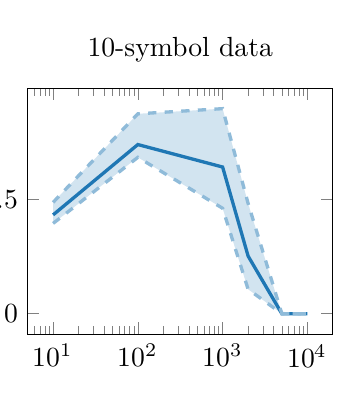
\begin{tikzpicture}[trim axis left, trim axis right]
\begin{semilogxaxis}[
  width=0.45\textwidth,
  title={10-symbol data},
  ytick={0,0.5,1}
]
  \addplot[cbblue,name path=median 1]
    coordinates{(10,   0.4333) (100,   0.7417) (1000, 0.6431) (2000, 0.2526)
                (5000, 0.0000) (10000, 0.0000)};
  \addplot[cbblue!50,dashed,name path=lower 1,forget plot]
    coordinates{(10,   0.3958) (100,   0.6856) (1000, 0.4623) (2000, 0.1070)
                (5000, 0.0000) (10000, 0.0000)};
  \addplot[cbblue!50,dashed,name path=upper 1,forget plot]
    coordinates{(10,   0.4882) (100,   0.8765) (1000, 0.8991) (2000, 0.4834)
                (5000, 0.0001) (10000, 0.0000)};
  \addplot[cbblue,fill opacity=0.2,forget plot]
    fill between[of=lower 1 and upper 1];
\end{semilogxaxis}
\end{tikzpicture}
\qquad
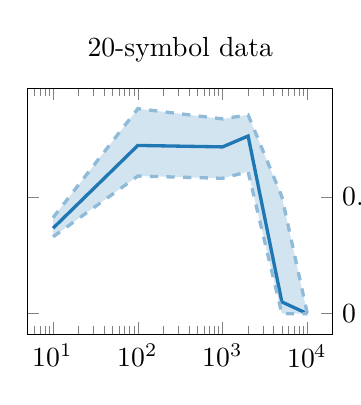
\begin{tikzpicture}[trim axis left, trim axis right]
\begin{semilogxaxis}[
  width=0.45\textwidth,
  title={20-symbol data},
  ytick={0,0.5,1},
  yticklabel pos=upper
]
  \addplot[cbblue,name path=median 1]
    coordinates{(10,   0.3658) (100,   0.7196) (1000, 0.7134) (2000, 0.7599)
                (5000, 0.0504) (10000, 0.0000)};
  \addplot[cbblue!50,dashed,name path=lower 1,forget plot]
    coordinates{(10,   0.3290) (100,   0.5887) (1000, 0.5791) (2000, 0.6074)
                (5000, 0.0000) (10000, 0.0000)};
  \addplot[cbblue!50,dashed,name path=upper 1,forget plot]
    coordinates{(10,   0.4108) (100,   0.8769) (1000, 0.8330) (2000, 0.8505)
                (5000, 0.5011) (10000, 0.0000)};
  \addplot[cbblue,fill opacity=0.2,forget plot]
    fill between[of=lower 1 and upper 1];
\end{semilogxaxis}
\end{tikzpicture}
\caption{Measurements of the maximum marginal probability of non-root model
  states for data sets of various sizes. Medians and quartiles derived from 20
  random sequences are shown for each model and each sequence
  length~\(\abs{\ub{x}}\).}
\label{fig:unstructured}
\end{figure}

The results depicted in Figure~\ref{fig:unstructured} are rather interesting:
although in the binary case the marginal probabilities of the non-trivial states
appear to decrease monotonically, and at a reasonable rate, the same cannot be
said of the 10- and 20-character models. For both of the larger models, the
maximum probability first \emph{increases} before finally decreasing, and the
values observed are often above~0.5, and occasionally near~1.

Although slightly unexpected, this behaviour is not difficult to explain: as the
number of symbols increases, the expected number of occurrences of each state in
a fixed-length sequence decreases. This implies that the empirical distributions
associated with these states---that is, the counts of the symbols that
immediately follow them in the sequence---are sparser. In addition, the chance
of at least one state having a markedly non-uniform distribution increases
naturally with the number of symbols. One also needs to take into account the
behaviour of each state's children (and their children, and so on), because the
empirical distributions associated with these states will influence the
estimated probabilities of their parents. Finally, the fact that the maximum
inferred probability appears to \emph{increase} at first is simply due to the
size of the first one or two data sets: they are too small for any non-uniform
behaviour to be of any real significance.

In the end it is a combination of the reasons given above that causes inference
on models with large symbol alphabets to converge relatively slowly (in terms of
data-set size). That being said, the traces shown in
Figure~\ref{fig:unstructured} tell a somewhat one-sided story: if one plots the
\emph{mean} marginal probability of the root's child nodes instead of the
maximum, one finds that in both the 10- and 20-character case, across all of the
tested sequence lengths, this mean never rises above~0.4. In both cases the
plots are then monotonically decreasing from~\(\abs{\ub{x}} = 100\) onwards.
Plots of the median probability behave similarly.

\subsubsection{Asymptotic rate of convergence}\label{sec:asymptotic} %==========

To end this section, we give a quick derivation of the asymptotic rate at which
the marginal likelihood decreases with each attachment operation of a full
binary tree, as a function of the sequence length~\(n = \abs{\ub{x}}\). The idea
here is to quantify, for large \(n\), the effect that adding all of a leaf
node's children to the model has on the marginal likelihood~\(\Pb(\ub{x} \mid
\mc{S})\).

Recall from~\eqref{eqn:bayes factor} that if \(\mc{S}'\) is the model created by
attaching a node to a leaf~\(r\) of the state tree~\(\mc{S}\), then the ratio of
the two models' marginal likelihoods is:
\begin{equation}
  \frac{\Pb\lr{\ub{x} \mid \mc{S}'}}{\Pb\lr{\ub{x} \mid \mc{S}}} =
    \frac{\Beta\lr{\ub{n}_r + \ub{\alpha} \mid \mc{S}'}}
    {\Beta\lr{\ub{n}_r + \ub{\alpha} \mid \mc{S}}}
    \frac{\Beta\lr{\ub{n}_{0r} + \ub{\alpha}}}{\Beta\lr{\ub{\alpha}}}.
\end{equation}
Here we have assumed that the newly attached node represents the symbol~0, and
have labelled it as state \(0r\) accordingly. A full binary attachment involves
the attachment of a node representing the symbol~1 as well, and the ratio
involving the resulting model~\(\mc{S}''\) is:
\begin{equation}\label{eqn:bayes factor binary}
  \frac{\Pb\lr{\ub{x} \mid \mc{S}''}}{\Pb\lr{\ub{x} \mid \mc{S}}} =
    \frac{\Beta\lr{\ub{n}_r + \ub{\alpha} \mid \mc{S}''}}
    {\Beta\lr{\ub{n}_r + \ub{\alpha} \mid \mc{S}}}
    \frac{\Beta\lr{\ub{n}_{0r} + \ub{\alpha}}\,
    \Beta\lr{\ub{n}_{1r} + \ub{\alpha}}}{\Beta\lr{\ub{\alpha}}^2}.
\end{equation}

If the data set in question is simply a sequence of symbols generated according
to the unstructured, uniform distribution~\(\Pb(x \peq 1) = 0.5\), then for
large enough~\(n\) the occurrence counts associated with any given state will be
roughly equal; that is, \(\ub{n}_s(0) \approx \ub{n}_s(1)\). (Technically we can
assume that~\(\ub{n}_s(1) - \ub{n}_s(0) = o(n)\), although we omit this from the
derivation below for the sake of brevity.) In particular, the counts
corresponding to the root state will satisfy~\(\ub{n}_{\lambda} \approx (n/2,
n/2)\) (recall that the root state represents the empty prefix, which `occurs'
before every symbol in the sequence); those associated with the root's child~0
will be~\(\ub{n}_0 \approx (n/4, n/4)\); and so on.

Let~\(r = \lambda\) in the above equations, so that \(\mc{S}\) and \(\mc{S}''\)
are now the complete binary state trees of sizes~1 and~3 respectively. Note also
that when both children of the root are present (in~\(\mc{S}''\)), the
state~\(\lambda\) will only have an effective count of~1, which we without loss
of generality assume corresponds to the symbol~0. Using idealised---but
asymptotically valid---counts, we have:
\begin{align}\label{eqn:bayes factor asymptotic}
  \frac{\Pb(\ub{x} \mid \mc{S}'')}{\Pb(\ub{x} \mid \mc{S})} &=
    \frac{\Beta(\ub{n}_{\lambda} + \ub{\alpha} \mid \mc{S}'')}
    {\Beta(\ub{n}_{\lambda} + \ub{\alpha} \mid \mc{S})}
    \frac{\Beta(\ub{n}_0 + \ub{\alpha})\, \Beta(\ub{n}_1 + \ub{\alpha})}
    {\Beta(\ub{\alpha})^2} \nonumber \\
  &\sim \frac{\Beta\lr*{\lr*{1, 0} + \ub{\alpha}}\,
    \Beta\lr*{\lr*{\frac{n}{4}, \frac{n}{4}} + \ub{\alpha}}\,
    \Beta\lr*{\lr*{\frac{n}{4}, \frac{n}{4}-1} + \ub{\alpha}}}
    {\Beta\lr*{\lr*{\frac{n}{2}, \frac{n}{2}} + \ub{\alpha}}\,
    \Beta(\ub{\alpha})^2}.
\end{align}

We can treat this equation in parts, starting with the constant terms. To
simplify the derivation we also assume that the concentration parameter is
symmetric:~\(\ub{\alpha} = (\alpha, \alpha, \dots)\).
\begin{align*}
  \frac{\Beta((1, 0) + \ub{\alpha})}{\Beta(\ub{\alpha})^2} &=
    \frac{\Gamma(1 + \alpha)\, \Gamma(\alpha)}{\Gamma(1 + 2\alpha)}
    \frac{\Gamma(2\alpha)}{\Gamma(\alpha)\, \Gamma(\alpha)}
    \frac{1}{\Beta(\ub{\alpha})} \\
  &= \frac{1}{2\Beta(\ub{\alpha})}.
\end{align*}

The terms that are dependent on~\(n\) can be simplified using Stirling's
formula, e.g.:
\begin{align*}
  \Beta\lr*{\lr*{\frac{n}{4}, \frac{n}{4}} + \ub{\alpha}} &\sim
    \sqrt{2\pi}\, \frac{\lr*{\frac{n}{4} + \alpha}^{(n/4)+\alpha-(1/2)}
    \lr*{\frac{n}{4} + \alpha}^{(n/4)+\alpha-(1/2)}}
    {\lr*{\frac{n}{2} + 2\alpha}^{(n/2)+2\alpha-(1/2)}} \\
  &\sim \sqrt{2\pi}\, \frac{\lr*{\frac{n}{4}}^{(n/4)+\alpha-(1/2)}
    \lr*{\frac{n}{4}}^{(n/4)+\alpha-(1/2)}}
    {\lr*{\frac{n}{2}}^{(n/2)+2\alpha-(1/2)}}.
\end{align*}
Applying this to the three dependent terms yields:
\begin{align*}
  \frac{\Beta\lr*{\lr*{\frac{n}{4}, \frac{n}{4}} + \ub{\alpha}}\,
    \Beta\lr*{\lr*{\frac{n}{4}, \frac{n}{4}-1} + \ub{\alpha}}}
    {\Beta\lr*{\lr*{\frac{n}{2}, \frac{n}{2}} + \ub{\alpha}}}
  &\sim \sqrt{2\pi}\, \frac{\lr*{\frac{n}{4}}^{3((n/4)+\alpha-(1/2))}
    \lr*{\frac{n}{4}}^{(n/4)+\alpha-(3/2)}}
    {\lr*{\frac{n}{2}}^{(n/2)+2\alpha-(1/2)}
    \lr*{\frac{n}{2}}^{(n/2)+2\alpha-(3/2)}} \\
  &\times \frac{n^{n+2\alpha-(1/2)}}
    {\lr*{\frac{n}{2}}^{2((n/2)+\alpha-(1/2))}} \\
  &= \sqrt{2\pi}\, \frac{\lr*{\frac{n}{4}}^{n+4\alpha-3} n^{n+2\alpha-(1/2)}}
    {\lr*{\frac{n}{2}}^{2n+6\alpha-3}} \\
  &= \sqrt{2\pi}\, 2^{3-2\alpha} n^{-1/2}.
\end{align*}

Putting the constant and dependent terms together, Equation~\eqref{eqn:bayes
factor asymptotic} reduces to:
\begin{equation}\label{eqn:bayes factor asymptotic 2}
  \frac{\Pb(\ub{x} \mid \mc{S}'')}{\Pb(\ub{x} \mid \mc{S})} \sim
    \frac{\sqrt{2\pi}}{\Beta(\ub{\alpha})} 4^{1-\alpha} n^{-1/2}.
\end{equation}
What this means is that in the case of uniformly random binary data, the
marginal likelihood of a three-node, complete state tree is smaller than that of
the single-node model by a factor that is~\(\Theta(n^{-1/2})\) for large~\(n =
\abs{\ub{x}}\). The same goes for larger state trees: attaching a pair of nodes
to a leaf of the three-node tree to form a five-node model will further reduce
the marginal likelihood by a factor of order~\((n/2)^{-1/2}\) (because roughly
half of the symbols in the sequence match the existing state), and so on.

Of course, in the previous sections we have not been dealing with the marginal
likelihoods of individual models; rather, we have been interested in \emph{sums}
of marginal likelihoods over models that include a particular node~\(s\).
Ideally, one would like to build on Equation~\ref{eqn:bayes factor asymptotic 2}
by deriving the (asymptotic) relative likelihood of any given tree, and then
normalising these relative values to yield an asymptotic version of the model
posterior.

Specifically, one might approximate the unnormalised likelihood of a binary tree
by noting that every node other than the root adds a factor~\(Cn^{-1/2}\) to
this likelihood, plus another factor~\(2^{r/2}\) based on the distance~\(r\) of
the node from the root. The relative likelihood of a full binary tree with~\(m\)
nodes is thus:
\begin{equation*}
  L(m,k) = C n^{-m/2} 2^{r/2},
\end{equation*}
where~\(k\) is the sum of the distances from each node to the root. This
distance sum is known as the `path length' of a tree, and has been studied
extensively for trees such as those discussed here (see, e.g.,
\cite[Section~3.5]{flajolet2009analytic}).

In general the idea is to enumerate the number of trees with~\(m\) nodes and
path length~\(k\) using a bivariate generating function in which the (unknown)
coefficient represents the count:
\begin{equation*}
  B(z, u) = \sum_{m\geq 0} \sum_{k\geq 0} b_{m,k} z^m u^k.
\end{equation*}
If such a generating function were available in closed form (for example, the
univariate generating function that counts the internal nodes of full binary
trees---with no regard for path length---is given by~\(B(z) = (1 - \sqrt{1 -
4z})/(2z)\)), one could derive the sum of~\(L(m, k)\) over all trees by the
simple substitution~\((z, u) = (n^{-1/2}, \sqrt{2})\).

Unfortunately, we do not know of such a closed form. In the case of the path
length of a tree, one usually makes use of the bivariate generating function for
the sake of moment analysis, which does not require an explicit closed form. In
any case, we have mentioned the idea here for interest's sake---and potential
future reference.

\section{Conclusion} %==========================================================

A number of topics have been discussed in this article: the marginal likelihood
of variable-order Markov models; the relationship between the posterior
distribution over such models and conditional independence; MCMC sampling over
this posterior, and its applications; and, briefly, the analysis of binary
Markov models in the face of unstructured data.

The inference of the marginal likelihood of a model in a Bayesian way is
particularly interesting, and its combination with Markov chain Monte Carlo
methods for the sake of model inference is also quite natural. In our
experiments, the states of high marginal probability inferred in this way mostly
line up well with the true model in the case of synthetic data, and with
intuition in the case of real-world data.

For the interested reader, there is obviously a wealth of information on the
topic of variable-order Markov models in the literature: from their introduction
and development by Rissanen and
others~\cite{rissanen1986complexity,willems1995context,cleary1984data,
begleiter2004prediction}---mostly for the purposes of compression and
prediction---to more modern, Bayesian
approaches~\cite{dimitrakakis2010bayesian,mochihashi2008infinite}. I should
point out however, that the purpose of this article was neither to reimplement
these techniques nor to outperform them, and that I am by no means an expert on
the topic.

\printbibliography

\end{document}